% ============================================================
%  MAIN.TEX --- Documento principal
%  Compilar con: XeLaTeX (por fontspec / Times New Roman)
% ============================================================

\documentclass[12pt, a4paper]{report}

% ============================================================
%  FUENTES Y CODIFICACIÓN (XeLaTeX)
% ============================================================
\usepackage{fontspec}
\setmainfont{Times New Roman}

% ============================================================
%  IDIOMA
% ============================================================
\usepackage[spanish]{babel}

% ============================================================
%  GEOMETRÍA DE PÁGINA
% ============================================================
\usepackage[a4paper, top=2cm, bottom=2.5cm, left=2.5cm, right=2.5cm]{geometry}

% ============================================================
%  TIPOGRAFÍA Y PÁRRAFOS
% ============================================================
\setlength{\parindent}{0pt}
\usepackage{parskip}

% ============================================================
%  COLORES
% ============================================================
\usepackage{xcolor}
\definecolor{azulprincipal}{RGB}{30, 70, 130}
\definecolor{naranjadestacado}{RGB}{210, 105, 30}
\definecolor{verdeclave}{RGB}{40, 120, 60}
\definecolor{grisclaro}{RGB}{245, 245, 245}
\definecolor{rojoriesgo}{RGB}{180, 30, 30}

% ============================================================
%  FORMATO DE TÍTULOS
%  \chapter en negro (estilo report), \section y abajo en color
% ============================================================
\usepackage{titlesec}

\titleformat{\chapter}[display]
  {\Large\bfseries}{}{0em}{}[\hrule height 1.5pt \vspace{0.5em}]

\titleformat{\section}
  {\large\bfseries\color{azulprincipal}}{}{0em}{}[\titlerule]

\titleformat{\subsection}
  {\normalsize\bfseries\color{naranjadestacado}}{}{0em}{}

\titleformat{\subsubsection}
  {\normalsize\bfseries\color{verdeclave}}{}{0em}{}

% ============================================================
%  TABLAS
% ============================================================
\usepackage{booktabs}
\usepackage{array}

% ============================================================
%  LISTAS
% ============================================================
\usepackage{enumitem}

% ============================================================
%  RECUADROS (mdframed, reemplaza tcolorbox para este estilo)
% ============================================================
\usepackage{mdframed}

% Recuadro azul: puntos clave
\newmdenv[
  backgroundcolor=grisclaro,
  linecolor=azulprincipal,
  linewidth=1.2pt,
  roundcorner=4pt,
  innerleftmargin=10pt,
  innerrightmargin=10pt,
  innertopmargin=8pt,
  innerbottommargin=8pt
]{cajakeypoints}

% Recuadro rojo: advertencias y riesgos
\newmdenv[
  backgroundcolor=rojoriesgo!8,
  linecolor=rojoriesgo,
  linewidth=1pt,
  roundcorner=4pt,
  innerleftmargin=10pt,
  innerrightmargin=10pt,
  innertopmargin=8pt,
  innerbottommargin=8pt
]{cajariesgo}

% Recuadro verde: definiciones formales
\newmdenv[
  backgroundcolor=verdeclave!8,
  linecolor=verdeclave,
  linewidth=1pt,
  roundcorner=4pt,
  innerleftmargin=10pt,
  innerrightmargin=10pt,
  innertopmargin=6pt,
  innerbottommargin=6pt
]{cajadefinicion}

% ============================================================
%  ENCABEZADO Y PIE DE PÁGINA
% ============================================================
\usepackage{fancyhdr}
\setlength{\headheight}{13.68802pt}
\pagestyle{fancy}
\fancyhf{}
\rhead{\small\color{gray} Imagenología Especializada I}
\lhead{\small\color{gray} \leftmark}   % muestra el nombre del capítulo activo
\cfoot{\thepage}

% ============================================================
%  IMÁGENES
% ============================================================
\usepackage{graphicx}

% ============================================================
%  COLUMNAS MÚLTIPLES
% ============================================================
\usepackage{multicol}

% ============================================================
%  MARCA DE AGUA
% ============================================================
\usepackage{draftwatermark}
\SetWatermarkText{Uso personal}
\SetWatermarkScale{0.6}
\SetWatermarkLightness{1}   % levemente visible, no tapona el texto

% ============================================================
%  HIPERVÍNCULOS (siempre al final del preámbulo)
% ============================================================
\usepackage{hyperref}
\hypersetup{
  colorlinks=true,
  linkcolor=blue!60!black,
  urlcolor=blue!60!black
}

% ============================================================
\begin{document}
% ============================================================

\title{\textbf{\color{azulprincipal} Resumen Imagenología Especializada I}}
\author{DC}
\date{2026}

\maketitle
\tableofcontents
\newpage

% ============================================================
%  CAPÍTULOS --- agrega un \input{} por cada tema nuevo
% ============================================================
% ============================================================
%  medios_de_contraste.tex --- SOLO CONTENIDO
%  No tiene \documentclass ni \begin{document}.
%  Se incluye desde main.tex con \input{medios_de_contraste}
% ============================================================

\chapter{Medios de Contraste}

% --- Datos del docente ---
{\normalsize\color{gray} Lic. Matías Prado \quad|\quad Lic. Mauro Canclini}
\vspace{1em}

% ============================================================
%  PUNTOS CLAVE PARA EL EXAMEN ORAL
% ============================================================
\begin{cajakeypoints}
\textbf{\color{azulprincipal} Puntos clave para el examen oral}
\begin{itemize}[noitemsep, topsep=2pt]
  \item Definición y finalidad diagnóstica/terapéutica de los MC.
  \item Triple clasificación: por tipo de imagen, vía de administración y método de imagen.
  \item Estructura química de los MCI: anillo de benceno, posición de los átomos de yodo.
  \item Propiedades fisicoquímicas: osmolaridad, ionicidad, estructura molecular, viscosidad.
  \item El contraste \textbf{ideal}: no iónico, dímero, isoosmolar $\Rightarrow$ menor incidencia de reacciones adversas.
  \item Reacciones adversas: fisicoquímicas (dosis-dependientes) vs.\ idiosincráticas (dosis-independientes).
  \item Clasificación por gravedad: leves (98\%), moderadas (1\%), graves (1\%).
  \item NIC: filtrado glomerular (FG) como predictor; umbrales de riesgo.
  \item Protocolo de extravasación: pasos ordenados.
  \item Gadolinio: paramagnético, quelante, fibrosis sistémica nefrogénica en insuficiencia renal.
  \item Consentimiento informado: deber médico y derecho del paciente.
  \item Situaciones especiales: embarazo y lactancia.
\end{itemize}
\end{cajakeypoints}

\vspace{1em}

% ============================================================
\section*{Definición}
% ============================================================

\begin{cajadefinicion}
Un \textbf{medio de contraste (MC)} es toda sustancia o combinación de sustancias que, introducida en el organismo por cualquier vía, \textbf{permite resaltar y opacificar estructuras anatómicas normales} (órganos, vasos) \textbf{y patológicas} (tumores). También evalúa la perfusión y diferencia interfases de densidad entre tejidos de forma \textit{temporal}, con fines médicos diagnósticos y/o terapéuticos.
\end{cajadefinicion}

La indicación del MC se justifica porque las \textbf{partes blandas poseen bajo contraste natural}, lo que hace necesaria la administración de sustancias que las diferencien. El MC se elige y adapta según la región a estudiar y la técnica de exploración.

% ============================================================
\section*{Clasificación}
% ============================================================

\subsection*{1. Por tipo de imagen}

\renewcommand{\arraystretch}{1.35}
\begin{center}
\begin{tabular}{>{\bfseries}p{2.8cm} p{5cm} p{5cm}}
\hline
Tipo & Mecanismo & Ejemplos \\
\hline
Positivos & Atenúan más los Rx que los tejidos blandos. Se ven \textbf{radiopacos} (blancos). & Bario, Yodo, Gadolinio$^*$ \\[0.5em]
\hline
Negativos & Atenúan menos los Rx que los tejidos blandos. Se ven \textbf{radiolúcidos} (negros). & Aire, CO$_2$ \\[0.5em]
\hline
Neutros & Distienden y rellenan el tubo digestivo sin modificar densidad. & Agua, Metilcelulosa, Polietilenglicol, Manitol \\
\hline
\multicolumn{3}{l}{\footnotesize $^*$El gadolinio no interactúa con los Rx; se emplea en resonancia magnética.}
\end{tabular}
\end{center}

\subsection*{2. Por vía de administración}

Intravenosa (EV), intraarterial, intracanalicular, intraarticular, intravaginal, rectal, oral, entre otras.

\subsection*{3. Por método de imagen}

\renewcommand{\arraystretch}{1.35}
\begin{center}
\begin{tabular}{>{\bfseries}p{2.5cm} p{9.5cm}}
\hline
Método & Tipo de contraste utilizado \\
\hline
Rx contrastada & Bario, aire/polvo efervescente (oral); Yodo (EV) \\
\hline
TC / TCMS & Bario, Agua, Yodo, Aire y CO$_2$, Metilcelulosa, Manitol, Polietilenglicol \\
\hline
RM & Gadolinio (EV e intraarticular), Metilcelulosa, Manitol, Polietilenglicol \\
\hline
PET & Radiotrazadores: 18-FDG, Carbono-11, Flúor-18, Indio-111 (EV) \\
\hline
Ultrasonido (US) & Microburbujas (EV) \\
\hline
Angiografía (AD) & Yodo/Gadolinio y CO$_2$ (arterial); Yodo (EV) \\
\hline
\end{tabular}
\end{center}

% ============================================================
\section*{Medios de Contraste Iodados (MCI)}
% ============================================================

El \textbf{anillo de benceno} es el sustrato básico. Requiere \textbf{tres átomos de yodo en un monómero} (seis en un dímero) para lograr opacidad radiológica adecuada.

\begin{itemize}[noitemsep]
  \item C2, C4, C6: átomos de \textbf{yodo}.
  \item C1: grupo carboxilo (-COOH) o hidroxilo (-OH).
  \item C3 y C5: radicales orgánicos (determinan \textit{solubilidad}, \textit{unión a proteínas} y \textit{vía de excreción}).
\end{itemize}

Excreción predominantemente \textbf{renal}. Vida media $\approx$ 1 hora en individuos sanos.

\subsection*{Clasificación fisicoquímica}

\renewcommand{\arraystretch}{1.35}
\begin{center}
\begin{tabular}{p{2.8cm} >{\centering}p{2.5cm} >{\centering}p{2.5cm} >{\centering}p{2.5cm} >{\centering\arraybackslash}p{2.5cm}}
\hline
\textbf{Propiedad} & \textbf{\color{rojoriesgo}Alta OSM} & \textbf{Baja OSM} & \textbf{Baja OSM} & \textbf{\color{verdeclave}Isoosmolar} \\
\hline
OSM (mOsm/kg) & $\sim$2100 & 577 & 600--900 & 290 \\
\hline
Ionicidad & Iónico & Iónico & No iónico & No iónico \\
\hline
Estructura & Monómero & Dímero & Monómero & Dímero \\
\hline
Viscosidad 37°C & 8,4 & 9,5 & 7,8--11,2 & 11,1 \\
\hline
Ejemplo & Diatrizoato & Hexabrix & Omnipaque, Xenetix & Visipaque \\
\hline
\end{tabular}
\end{center}

\begin{cajakeypoints}
\textbf{Concepto clave:} Los contrastes \textbf{no iónicos, dímeros e isoosmolares} presentan \textbf{menor incidencia de reacciones adversas}. Esto no implica que sean los más comercializados.
\end{cajakeypoints}

\subsubsection*{Viscosidad}
Resistencia de los fluidos a la circulación. \textbf{Relación inversa} con temperatura y osmolaridad (se calientan a 37°C). \textbf{Relación directa} con tamaño molecular, lo que influye en la quimiotoxicidad.

% ============================================================
\section*{Gadolinio (Gd)}
% ============================================================

Metal \textbf{paramagnético} de la familia de los lantánidos. Acelera el tiempo de relajación (TR) en RM. \textbf{Aumenta la señal en T1} y la \textbf{disminuye en T2}. En forma libre es tóxico; se neutraliza con un \textbf{agente quelante}. Excreción \textbf{renal}.

\begin{itemize}[noitemsep]
  \item \textbf{Quelante lineal}: menor estabilidad, mayor riesgo de Gd libre (\textit{transmetilación}).
  \item \textbf{Quelante cíclico}: mayor estabilidad termodinámica. \textbf{Preferido clínicamente.}
\end{itemize}

% ============================================================
\section*{Reacciones Adversas}
% ============================================================

\subsection*{Por fisiopatología}

\subsubsection*{Fisicoquímicas o quimiotóxicas}
\textbf{Dosis-dependientes.} Acción directa sobre células, tejidos y sistemas enzimáticos. En vasos: daño endotelial, deformación de glóbulos rojos, trombosis.

\subsubsection*{Idiosincráticas o por hipersensibilidad}
\textbf{Independientes de la dosis. Impredecibles.}
\begin{itemize}[noitemsep]
  \item \textbf{Inmediata}: dentro de los \textbf{60 minutos} posteriores.
  \item \textbf{Tardía}: entre \textbf{3 horas y 2 días}; se autolimitan en 1 a 7 días.
\end{itemize}

\subsection*{Por gravedad}

\renewcommand{\arraystretch}{1.35}
\begin{center}
\begin{tabular}{>{\bfseries}p{2.2cm} p{1.8cm} p{4.5cm} p{5cm}}
\hline
Gravedad & Frec. & Manejo & Manifestaciones \\
\hline
\color{verdeclave}Leves & 98\% & Autolimitadas. Observación. & Náuseas, vómitos leves, mareos, exantema, congestión nasal. \\[0.5em]
\hline
\color{naranjadestacado}Moderadas & $\sim$1\% & Requieren tratamiento. & Broncoespasmo, disnea, taquicardia, urticaria extensa, hipotensión. \\[0.5em]
\hline
\color{rojoriesgo}Graves & $\sim$1\% & Tratamiento e internación. & Edema laríngeo, shock, paro cardiorrespiratorio, convulsiones. \\
\hline
\end{tabular}
\end{center}


\begin{cajariesgo}
\textbf{Importante:} El calor, el deseo de orinar y el gusto metálico son \textbf{respuestas fisiológicas normales}, no reacciones adversas leves.
\end{cajariesgo}

\subsection*{Reacciones adversas del Gadolinio}

\begin{cajariesgo}
\textbf{Fibrosis Sistémica Nefrogénica (FSN):} reacción adversa \textit{exclusiva} del gadolinio. Solo en pacientes con \textbf{insuficiencia renal grave}. Presenta dolor generalizado, prurito, eritema y edema de tejidos blandos.
\end{cajariesgo}

% ============================================================
\section*{Factores de Riesgo}
% ============================================================

\begin{itemize}[noitemsep]
  \item Reacción alérgica previa al MC (\textbf{5 veces} más riesgo).
  \item Asma bronquial (\textbf{6 a 10 veces} más riesgo).
  \item Cualquier tipo de alergia (\textbf{3 veces} más riesgo).
  \item Hipertiroidismo, ansiedad, nefrópatas, diabéticos, cardiópatas.
  \item \textbf{Contraindicaciones absolutas:} mieloma múltiple, feocromocitoma, deshidratación.
\end{itemize}

\textbf{Prevención:} interrogatorio, consentimiento informado, ayuno 4 horas, hidratación, creatinina en mayores de 60 años (umbral: $>$1,1 mg/dl en mujeres; $>$1,3 mg/dl en hombres).

\clearpage

% ============================================================
\section*{Nefropatía Inducida por Contraste (NIC)}
% ============================================================

\begin{cajadefinicion}
La \textbf{NIC} es un \textit{rápido deterioro de la función renal} luego de la administración de MC. Principal predictor: \textbf{disfunción renal previa}.
\end{cajadefinicion}

{\renewcommand{\arraystretch}{1.35}
\begin{center}
\begin{tabular}{>{\bfseries}p{3.5cm} p{3cm} p{6cm}}
\hline
FG (ml/min) & Riesgo & Conducta \\
\hline
$>$ 60 & Bajo & Sin profilaxis. \\
\hline
30 -- 60 & Moderado & Tratamiento preventivo. \\
\hline
$<$ 30 & Elevado & Tratamiento preventivo intensivo. \\
\hline
$<$ 15 & Máximo & Evaluación por nefrología; posible diálisis. \\
\hline
\end{tabular}
\end{center}


% ============================================================
\section*{Extravasación de MC}
% ============================================================

Salida del MC del vaso hacia los tejidos blandos. Síntomas: dolor, hinchazón, hematoma, ulceración, síndrome compartimental.

\textbf{Mecanismos de daño:} osmolaridad (a mayor OSM, mayor daño), citotoxicidad (mayor en iónicos), volumen (a mayor volumen, mayor daño), compresión mecánica.

\subsection*{Protocolo de actuación}
\begin{enumerate}[noitemsep]
  \item Retirar la vía.
  \item Estimar el volumen extravasado (remanente en la bomba).
  \item Detectar la zona y drenar. \textbf{No masajear.}
  \item Elevar el miembro afectado por encima del corazón.
  \item Aplicar hielo.
  \item Observar y documentar hasta mejoría.
  \item Si síntomas progresan luego de \textbf{2 a 4 horas}: consulta con cirujano.
\end{enumerate}

% ============================================================
\section*{Consentimiento Informado}
% ============================================================

El paciente \textbf{decide y autoriza de forma consciente, libre y responsable}. Requiere explicación oral y escrita, sin coacción. Debe ser impreso, sin abreviaturas ni enmendaduras, y firmado por el paciente o su representante legal.

Es un \textbf{deber del médico} y un \textbf{derecho del paciente}.

\clearpage

% ============================================================
\section*{Situaciones Especiales}
% ============================================================

\subsection*{Embarazo}
Gadolinio y MCI \textbf{atraviesan la barrera placentaria}. Evitar salvo necesidad absoluta. Riesgo conocido con MCI: \textbf{depresión de la función tiroidea fetal}.

\subsection*{Lactancia}
Menos del \textbf{1\%} de la dosis se excreta en leche materna; de ese porcentaje, menos del 1\% es absorbido por el lactante. Precaución: amamantar antes de la inyección y extraer leche previamente para el siguiente amamantamiento.

% ============================================================
\section*{Bomba Inyectora}
% ============================================================

Inyección segura y reproducible. Parámetros: volumen (ml), flujo (ml/s), presión (PSI), \textit{rise time} (s). Útil en TC, RM y AD.

\textbf{Secuencia de armado:}
\begin{enumerate}[noitemsep]
  \item Introducir vaso con jeringa en el cabezal.
  \item Subir el pistón hasta arriba.
  \item Colocar prolongador para rellenar.
  \item Rellenar contraste.
  \item Rellenar suero (dilución si monocabezal).
  \item Purgar el sistema.
  \item Orientar la bomba hacia abajo.
  \item Introducir los valores de inyección.
\end{enumerate}

% ============================================================
\section*{Esquema Mental --- Repaso Final}
% ============================================================

\begin{cajakeypoints}
\begin{center}
\textbf{\color{azulprincipal}
  MC $\rightarrow$ 3 clasificaciones $\rightarrow$ MCI: anillo bencénico $\rightarrow$ propiedades fisicoquímicas}\\[0.4em]
\textbf{\color{naranjadestacado}
  Mejor MC: no iónico + dímero + isoosmolar (Visipaque)}\\[0.3em]
\textbf{\color{rojoriesgo}
  RA: fisicoquímica (dosis) vs.\ idiosincrática (impredecible)}\\[0.3em]
Leves 98\% \quad Moderadas $\sim$1\% \quad Graves $\sim$1\%\\[0.3em]
\textbf{NIC}: FG $<$ 60 $\Rightarrow$ profilaxis \quad FG $<$ 15 $\Rightarrow$ nefrología\\[0.3em]
\textbf{Extravasación}: retirar vía $\to$ elevar $\to$ no masajear $\to$ hielo\\[0.3em]
\textbf{Gd}: paramagnético, quelante cíclico, FSN solo en insuf.\ renal grave
\end{center}
\end{cajakeypoints}

\vspace{1em}
\hrule
\vspace{0.5em}
{\footnotesize \textit{Fuente: material de clase --- Imagenología Especializada I, Lic. Prado y Lic. Canclini, UdelaR 2026.}}
% ============================================================
%  CISTOGRAFÍA / CISTOURETROGRAFÍA
%  Licenciatura en Imagenología --- UdelaR
%  Imagenología Especializada I, 2026
%  Lic. Camila Mier
%
%  IMPORTANTE: Este archivo NO tiene \documentclass ni
%  \begin{document}. Todo eso vive en main.tex.
%  Compila siempre desde main.tex con XeLaTeX.
% ============================================================

\chapter{Cistografia}



% ============================================================
%  PUNTOS CLAVE PARA EL EXAMEN ORAL
% ============================================================
\begin{cajakeypoints}
\textbf{\color{azulprincipal} Puntos clave para el examen oral}
\begin{itemize}[noitemsep, topsep=2pt]
  \item Es una exploración radiológica del \textbf{tracto urinario inferior}: vejiga y uretra.
  \item La uretra femenina mide \textbf{4 cm}; la masculina varía entre \textbf{17,5 y 20 cm} (anterior: peneana + bulbar; posterior: prostática + membranosa).
  \item Se requiere \textbf{urocultivo negativo 72 horas antes} del estudio.
  \item Contraindicaciones absolutas: \textbf{infección aguda}, obstrucción uretral completa y embarazo.
  \item Sonda Foley: calibre \textbf{12--18 F} en adultos, \textbf{5--8 F} en niños. En el hombre se fija en la \textbf{fosa navicular} inflando el balón con \textbf{1--1,5 mL} de solución salina.
  \item Volumen de contraste yodado hidrosoluble: \textbf{400--450 mL}.
  \item Residuo post-miccional \textbf{mayor al 30\%} del volumen inicial se considera anormal.
  \item La estenosis de uretra anterior se valora en \textbf{fase de llenado}; la de uretra posterior en \textbf{proyecciones transmiccionales}.
\end{itemize}
\end{cajakeypoints}

\vspace{1em}

% ============================================================
%  SECCIÓN 1 --- DEFINICIÓN
% ============================================================
\section*{Definición}

\begin{cajadefinicion}
La \textbf{cistografía} (o cistouretrografía) es una exploración radiológica del tracto urinario inferior que permite estudiar la vejiga y la uretra mediante instilación retrógrada de contraste yodado hidrosoluble a través de una sonda vesical.
\end{cajadefinicion}

El estudio se practica preferentemente en varones para estudiar la totalidad de la uretra, aunque también se realiza en mujeres. Continúa siendo el \textbf{método diagnóstico inicial} para muchas enfermedades del sistema urinario inferior debido a su fácil acceso, bajo costo y gran exactitud.

% ============================================================
%  SECCIÓN 2 --- ANATOMÍA DE REFERENCIA
% ============================================================
\section*{Anatomía de Referencia}

\subsection*{Uretra femenina}

La uretra femenina mide aproximadamente \textbf{4 cm} de largo y se extiende desde el cuello de la vejiga en la unión ureterovesical hasta el vestíbulo, donde forma el meato externo entre los labios menores.

\subsection*{Uretra masculina}

La uretra masculina varía de \textbf{17,5 a 20 cm} de longitud y se divide en dos segmentos principales:

{\renewcommand{\arraystretch}{1.35}
\begin{center}
\begin{tabular}{>{\bfseries}p{3cm} p{4cm} p{6.5cm}}
\hline
Segmento & División & Porción \\
\hline
Posterior & Preprostática & Cuello vesical hasta próstata. \\[0.3em]
\hline
          & Prostática     & Atraviesa la próstata. \\[0.3em]
\hline
          & Membranosa     & Porción más corta; atraviesa el diafragma urogenital. \\[0.5em]
\hline
Anterior  & Bulbar         & Desde la membrana perineal hasta el pene. \\[0.3em]
\hline
          & Peneana        & Recorre el cuerpo del pene hasta la fosa navicular. \\
\hline
\end{tabular}
\end{center} 
}

% ============================================================
%  SECCIÓN 3 --- INDICACIONES
% ============================================================
\section*{Indicaciones}

\subsection*{Patológicas}

\begin{itemize}[noitemsep]
  \item Valoración de \textbf{estenosis}, estrecheces, traumatismos y tumores.
  \item \textbf{Reflujo vesicoureteral}.
  \item Infecciones urinarias recurrentes.
  \item Trastornos neurogénicos.
  \item Anomalías anatómicas.
  \item \textbf{Divertículos vesicales} (más frecuentes en la mujer).
  \item Incontinencia urinaria.
  \item Fístulas desde el aparato urinario al genital, digestivo o a la piel.
  \item Defecto de llenado.
  \item Hematuria.
\end{itemize}

% ============================================================
%  SECCIÓN 4 --- PREPARACIÓN Y CONTRAINDICACIONES
% ============================================================
\section*{Preparación Previa y Contraindicaciones}

\subsection*{Preparación previa}

El estudio \textbf{no requiere ayuno ni preparación intestinal}. Los pasos previos obligatorios son:

\begin{enumerate}[noitemsep]
  \item Realizar \textbf{urocultivo 72 horas antes}; el resultado debe ser negativo.
  \item Interrogar al paciente sobre \textbf{alergias} a medios de contraste, medicamentos o alimentos.
  \item Obtener \textbf{consentimiento informado} firmado.
\end{enumerate}

\clearpage

\subsection*{Contraindicaciones}

\begin{cajariesgo}
\textbf{Contraindicaciones absolutas:}
\begin{itemize}[noitemsep, topsep=2pt]
  \item Infección en período agudo (el urocultivo positivo es criterio de exclusión).
  \item Obstrucción uretral completa.
  \item Embarazo.
\end{itemize}
\end{cajariesgo}

% ============================================================
%  SECCIÓN 5 --- PROTOCOLO DE PROCEDIMIENTO
% ============================================================
\section*{Protocolo de Procedimiento}

\subsection*{Posición del paciente y preparación}

El paciente debe \textbf{orinar} antes de comenzar el estudio para vaciar la vejiga. A continuación se posiciona en \textbf{decúbito supino} sobre la mesa radiográfica.

\subsection*{Sondaje vesical}

\begin{enumerate}[noitemsep]
  \item Limpieza de genitales con \textbf{antiséptico}.
  \item Aplicación de \textbf{xilocaína en gel al 2\%} (anestésico local) en el meato uretral.
  \item Introducción de \textbf{sonda Foley}: calibre \textbf{12--18 F} en adultos y \textbf{5--8 F} en niños.
  \item \textbf{Fijación de la sonda:}
    \begin{itemize}[noitemsep]
      \item \textit{Hombres:} se fija a la altura de la \textbf{fosa navicular} inflando el balón con \textbf{1--1,5 mL} de solución salina.
      \item \textit{Mujeres:} se introduce hasta la luz de la vejiga y se fija directamente.
    \end{itemize}
  \item Instilación de \textbf{contraste yodado hidrosoluble} a través de la sonda, hasta un volumen de \textbf{400--450 mL}, hasta llenar la vejiga.
\end{enumerate}

\clearpage
% ============================================================
%  SECCIÓN 6 --- PROYECCIONES RADIOLÓGICAS
% ============================================================
\section*{Proyecciones Radiológicas}

Las proyecciones se realizan en el siguiente orden secuencial:

{\renewcommand{\arraystretch}{1.35}
\begin{center}
\begin{tabular}{>{\bfseries}p{3.5cm} p{4.5cm} p{5.5cm}}
\hline
Proyección & Momento & Lo que se evalúa \\
\hline
Aparato urinario simple & Previo al contraste & Cuerpos extraños, calcificaciones, alteraciones óseas. \\[0.5em]
\hline
Uretra & Fase de llenado & Anatomía uretral; estenosis de uretra anterior. \\[0.5em]
\hline
AP de pelvis (llenado parcial) & Durante el llenado & Ureteroceles y tumores (que podrían no verse con vejiga llena). \\[0.5em]
\hline
AP de pelvis (vejiga llena) supino y de pie & Vejiga llena & Morfología vesical, paredes, defectos de llenado, capacidad, descenso del piso; reflujo vesicoureteral en mujeres (fluoroscopia). \\[0.5em]
\hline
Oblicuas a 45° & Durante la micción & Unión vesicoureteral en busca de reflujo; márgenes vesicales. \\[0.5em]
\hline
Lateral & Durante la micción & Ángulos uretrales, descenso vesical; indicada en sospecha de incontinencia urinaria o fístulas (principalmente en mujeres). \\[0.5em]
\hline
Post-miccional & Tras la micción & Verificación de eliminación del contraste; residuo $>$30\% es anormal. Fluoroscopia de riñones para descartar reflujo. \\
\hline
\end{tabular}
\end{center}
}

\begin{figure}[h]
    \centering
    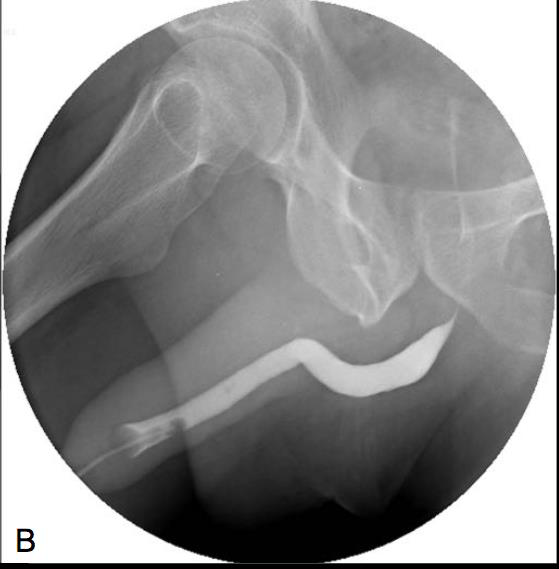
\includegraphics[width=0.5\linewidth]{imagenes/cisto1.png}
    \caption{Uretra durante llenado}
    \label{fig:c1}
\end{figure}

\begin{figure}
    \centering
    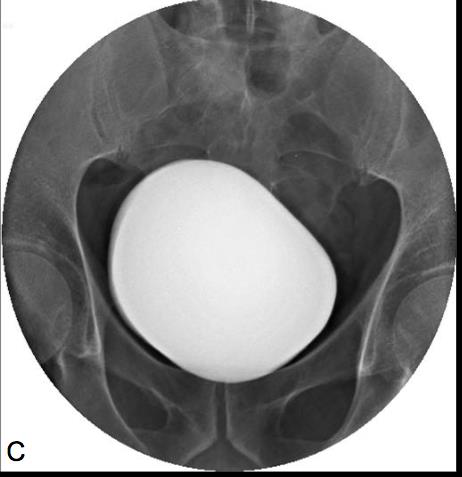
\includegraphics[width=0.5\linewidth]{imagenes/Cisto 2.png}
    \caption{Vejiga llena}
    \label{fig:c2}
\end{figure}

\begin{figure}
    \centering
    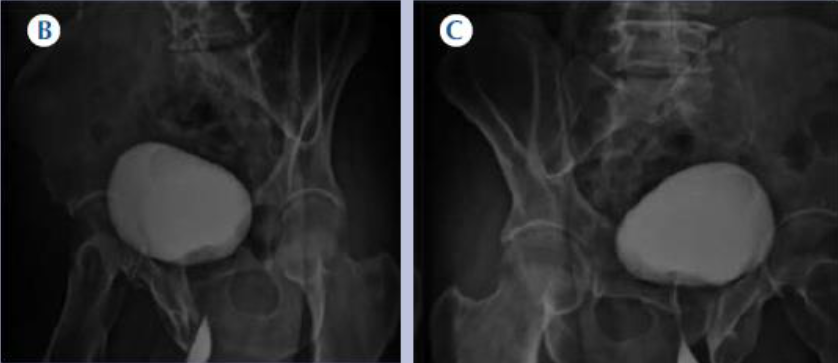
\includegraphics[width=1\linewidth]{imagenes/cisto4.png}
    \caption{Oblicuas, B derecha, C izquierda}
    \label{fig:c3}
\end{figure}

\begin{figure}
    \centering
    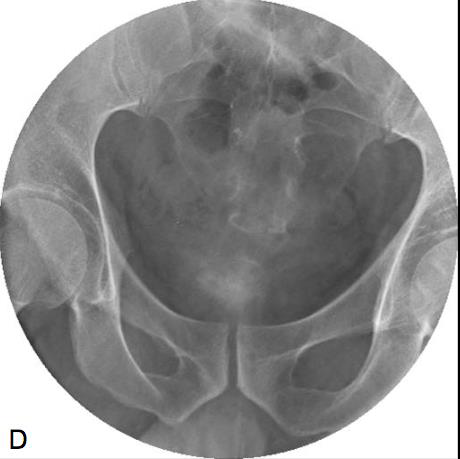
\includegraphics[width=0.5\linewidth]{imagenes/cisto5.png}
    \caption{Post micción}
    \label{fig:c4}
\end{figure}

\clearpage
% ============================================================
%  SECCIÓN 7 --- HALLAZGOS PATOLÓGICOS
% ============================================================
\section*{Hallazgos Patológicos Principales}

\subsection*{Estenosis uretral}

La estenosis restringe el flujo de orina desde la vejiga y puede generar inflamación o infección del tracto urinario. Es más frecuente en los \textbf{hombres} debido a la mayor longitud de la uretra.\\


\begin{cajakeypoints}
\textbf{Regla de valoración:} Uretra anterior $\to$ fase de \textbf{llenado}. \quad Uretra posterior $\to$ proyecciones \textbf{transmiccionales}.
\end{cajakeypoints}

\begin{figure}[h]
    \centering
    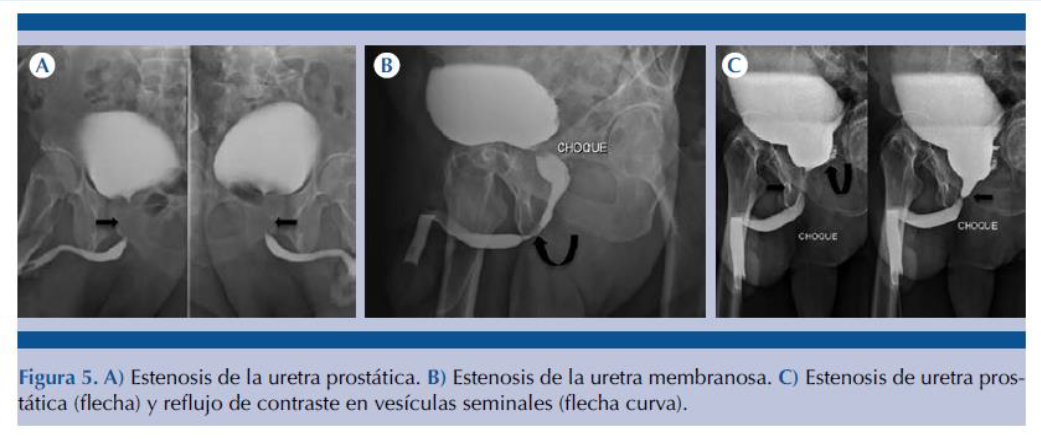
\includegraphics[width=1\linewidth]{imagenes/cisto estenosis.png}
    \caption{Estenosis}
    \label{fig:placeholder}
\end{figure}

\subsection*{Reflujo vesicoureteral}

Flujo anormal de orina que asciende de forma retrógrada desde la vejiga hacia el sistema urinario superior. Puede desencadenar infecciones urinarias recurrentes y, en su evolución, \textbf{falla renal}. Se detecta con fluoroscopia durante el llenado y la micción.

\begin{figure}[h]
    \centering
    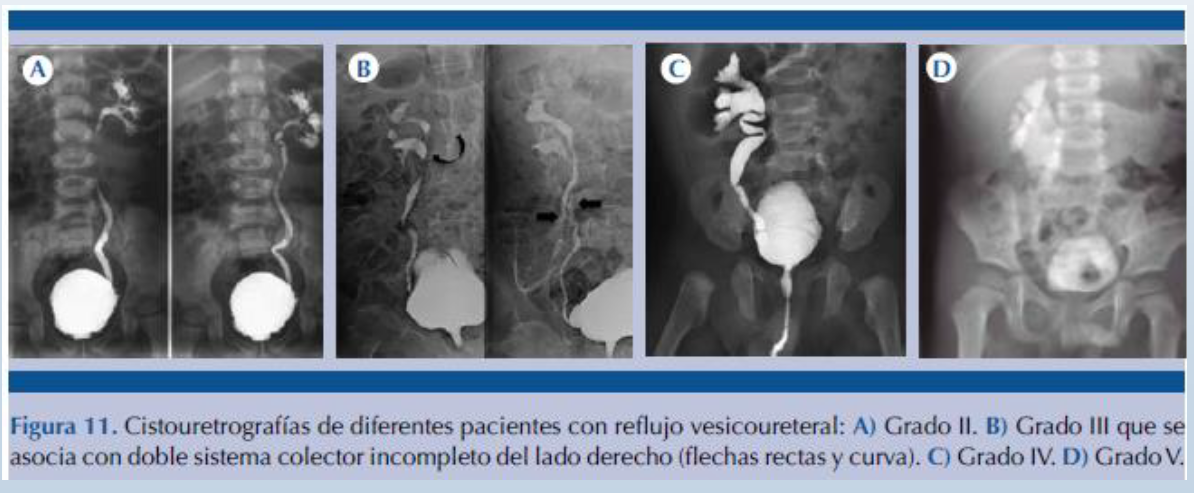
\includegraphics[width=1\linewidth]{imagenes/cisto reflujo.png}
    \caption{Reflujo vesicoureteral}
    \label{fig:c5}
\end{figure}

\subsection*{Fístulas del tracto genitourinario}

Comunicaciones anómalas entre la vejiga y estructuras adyacentes (vagina, recto, piel). Se evidencian con contraste en la proyección lateral durante la micción o en las oblicuas, como opacificación de estructuras ajenas al tracto urinario.

\begin{figure}[h]
    \centering
    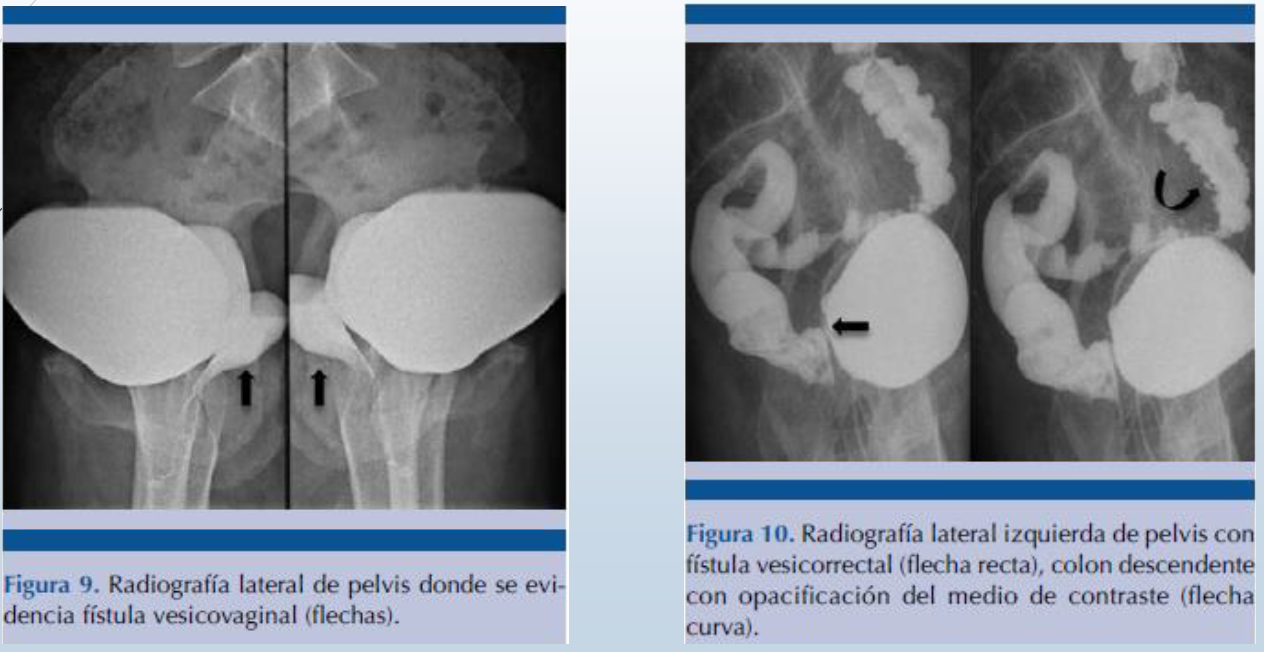
\includegraphics[width=1\linewidth]{imagenes/cisto fistulas.png}
    \caption{Fistulas}
    \label{fig:c6}
\end{figure}

\subsection*{Divertículo vesical}

Herniaciones de la mucosa vesical a través de la pared muscular de la vejiga. Aparecen como protrusiones saculares opacificadas con contraste adyacentes a la silueta vesical.

\begin{figure}
    \centering
    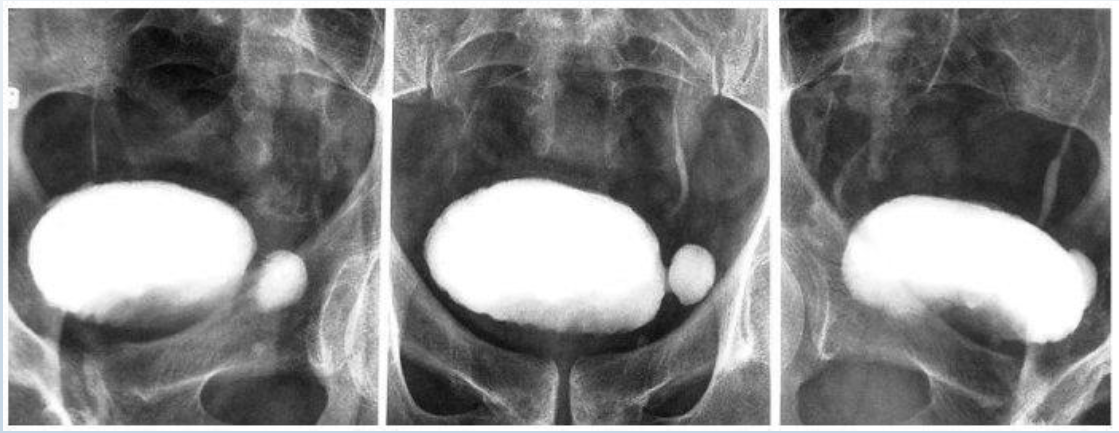
\includegraphics[width=1\linewidth]{imagenes/diverticulo.png}
    \caption{Diverticulo}
    \label{fig:c7}
\end{figure}

\subsection*{Cistocele e incontinencia urinaria}

Descenso de la vejiga con protrusión hacia la pared vaginal por debilidad del suelo pélvico. En la radiografía lateral (con maniobra de Valsalva o esfuerzo), la vejiga desciende por debajo del borde inferior de la sínfisis púbica. Se valoran los \textbf{ángulos uretrales} en la proyección lateral durante la micción.

\begin{figure}[h]
    \centering
    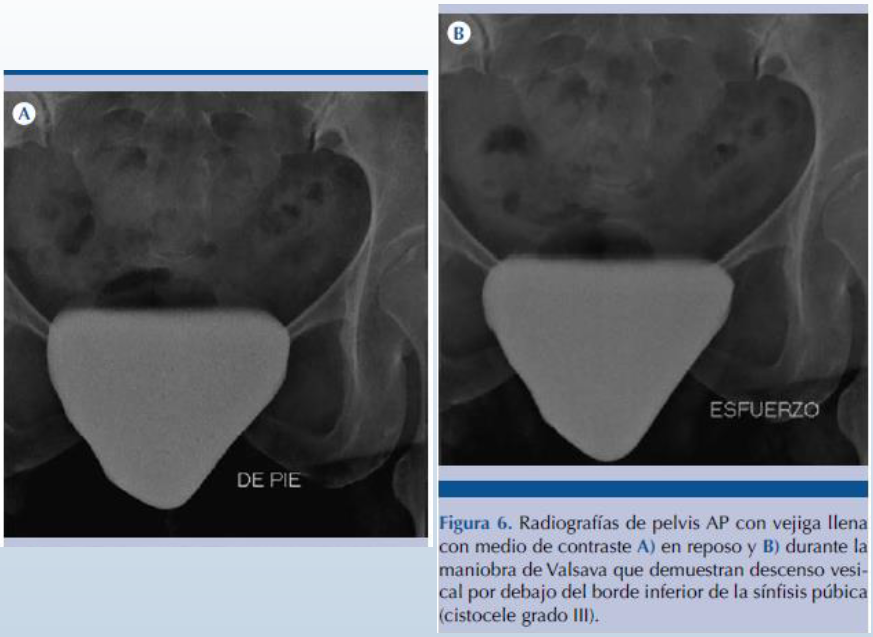
\includegraphics[width=1\linewidth]{cistocele.png}
    \caption{Cistocele}
    \label{fig:c8}
\end{figure}

\clearpage

% ============================================================
%  CIERRE --- ESQUEMA MENTAL FINAL
% ============================================================
\section*{Esquema Mental --- Repaso Final}

\begin{cajakeypoints}
\begin{center}
\textbf{\color{azulprincipal}
  Urocultivo negativo (72 h) $\rightarrow$ Sonda Foley $\rightarrow$ Contraste 400--450 mL $\rightarrow$ Serie de proyecciones $\rightarrow$ Post-miccional}\\[0.4em]
\textbf{\color{naranjadestacado}
  Residuo post-miccional $>$ 30\% = anormal. Estenosis anterior: llenado. Estenosis posterior: transmiccional.}\\[0.3em]
Uretra femenina: 4 cm \quad Uretra masculina: 17,5--20 cm \quad Sonda adulto: 12--18 F \quad Balón en hombre: 1--1,5 mL\\[0.3em]
\textbf{Protocolo:} simple $\to$ llenado AP $\to$ vejiga llena AP/oblicuas $\to$ miccional lateral $\to$ post-miccional
\end{center}
\end{cajakeypoints}

\vspace{1em}
\hrule
\vspace{0.5em}
{\footnotesize \textit{Fuente: material de clase --- Imagenología Especializada I, UdelaR 2026. Lic. Camila Mier.}}
% ============================================================
%  HISTEROSALPINGOGRAFÍA (HSG)
%  Licenciatura en Imagenología --- UdelaR
%  Imagenología Especializada I, 2026
%  Lic. Camila Mier
%
%  IMPORTANTE: Este archivo NO tiene \documentclass ni
%  \begin{document}. Todo eso vive en main.tex.
%  Compila siempre desde main.tex con XeLaTeX.
% ============================================================

\chapter{Histeosalpingogrfia (HSG)}

% ============================================================
%  PUNTOS CLAVE PARA EL EXAMEN ORAL
% ============================================================
\begin{cajakeypoints}
\textbf{\color{azulprincipal} Puntos clave para el examen oral}
\begin{itemize}[noitemsep, topsep=2pt]
  \item La HSG es el \textbf{Gold Standard} para estudio de infertilidad: evalúa morfología uterina y \textbf{permeabilidad tubárica}.
  \item Se realiza en la \textbf{fase folicular}, entre el \textbf{7° y 12° día} del ciclo menstrual (endometrio delgado, riesgo de embarazo casi nulo).
  \item Requiere \textbf{BHCG negativa} antes del estudio.
  \item Catéter utilizado: \textbf{sholkoff 5--7 Fr}; el balón se infla a nivel del \textbf{istmo} con una jeringa de \textbf{10 mL de aire}.
  \item Volumen de contraste yodado hidrosoluble: aproximadamente \textbf{10 cc}.
  \item Contraindicaciones: infección genital activa, embarazo, lactancia.
  \item Útero bicorne: ángulo intercornual \textbf{$>$ 105°}. Útero septado: ángulo intercornual \textbf{$<$ 75°}.
  \item El paso bilateral de contraste a la cavidad peritoneal confirma la \textbf{permeabilidad tubárica bilateral}.
\end{itemize}
\end{cajakeypoints}

\vspace{1em}

% ============================================================
%  SECCIÓN 1 --- DEFINICIÓN
% ============================================================
\section*{Definición}

\begin{cajadefinicion}
La \textbf{histerosalpingografía (HSG)} es una prueba diagnóstica que consiste en la administración de contraste yodado a través del cuello cervical para evaluar la morfología de la cavidad uterina y el funcionalismo de las trompas de Falopio.
\end{cajadefinicion}

Durante muchos años ha sido la prueba de elección para el estudio de la morfología y funcionalismo de las trompas de Falopio. Con un correcto conocimiento anatómico y una buena calidad técnica permite también una adecuada evaluación de la \textbf{cavidad uterina} y el diagnóstico diferencial entre variantes de la normalidad y hallazgos patológicos.

\clearpage

% ============================================================
%  SECCIÓN 2 --- ANATOMÍA DE REFERENCIA
% ============================================================
\section*{Anatomía de Referencia}

Las estructuras que se opacifican durante la HSG son:

\begin{itemize}[noitemsep]
  \item \textbf{Cuello del útero} (cérvix): punto de entrada del catéter.
  \item \textbf{Cuerpo del útero}: cavidad principal evaluada.
  \item \textbf{Fundus del útero}: fondo uterino; su morfología orienta el diagnóstico de malformaciones.
  \item \textbf{Cuernos uterinos}: unión entre la cavidad y el origen de cada trompa.
  \item \textbf{Trompas de Falopio}: compuestas por istmo y ampolla; su permeabilidad es el objetivo principal del estudio.
  \item \textbf{Cavidad peritoneal}: la fuga bilateral de contraste confirma la permeabilidad tubárica completa.
\end{itemize}

% ============================================================
%  SECCIÓN 3 --- INDICACIONES Y DATOS CLÍNICOS
% ============================================================
\section*{Indicaciones y Datos Clínicos}

\subsection*{Indicaciones patológicas}

\begin{itemize}[noitemsep]
  \item \textbf{Estudio de la infertilidad} (malformación uterina y permeabilidad tubárica --- Gold Standard).
  \item Abortos de repetición.
  \item Malformaciones congénitas uterinas.
  \item Valoración \textbf{pre y post-quirúrgica}, especialmente de la ligadura de trompas.
  \item Hemorragia uterina anormal.
  \item Poscesárea.
  \item Embarazo tubárico (luego de salpingotomía).
  \item Post-miomectomía (adherencias intrauterinas).
\end{itemize}

% ============================================================
%  SECCIÓN 4 --- PREPARACIÓN Y CONTRAINDICACIONES
% ============================================================
\section*{Preparación Previa y Contraindicaciones}

\subsection*{Verificaciones previas obligatorias}

\begin{enumerate}[noitemsep]
  \item Verificar que la paciente \textbf{no esté embarazada} (BHCG negativa).
  \item Interrogar sobre \textbf{antecedentes de infecciones genitales}.
  \item Evaluar \textbf{reacción alérgica} al medio de contraste yodado; algunos pacientes requieren preparación previa.
  \item Confirmar que el estudio se realiza en la \textbf{fase folicular} (entre el 7° y el 12° día del ciclo menstrual).
  \item Obtener \textbf{consentimiento informado} firmado.
\end{enumerate}

El procedimiento se realiza de modo \textbf{ambulatorio} y es muy rápido.

\clearpage

\subsection*{Contraindicaciones}

\begin{cajariesgo}
\textbf{Contraindicaciones absolutas:}
\begin{itemize}[noitemsep, topsep=2pt]
  \item Infección genital activa.
  \item Embarazo (BHCG positiva).
  \item Lactancia.
\end{itemize}
\end{cajariesgo}

\clearpage
% ============================================================
%  SECCIÓN 5 --- PROTOCOLO DE PROCEDIMIENTO
% ============================================================
\section*{Protocolo de Procedimiento}

\subsection*{Posición de la paciente}

La paciente se acuesta sobre la mesa de radiología digital en \textbf{decúbito supino en posición ginecológica}.

\subsection*{Pasos del procedimiento}

\begin{enumerate}[noitemsep]
  \item Desinfección del \textbf{periné y genitales externos}.
  \item Introducción del \textbf{espéculo}, eventualmente lubricado con vaselina.
  \item Desinfección del \textbf{cuello del útero} con solución antiséptica aplicada con pinzas y compresas.
  \item Introducción del \textbf{catéter sholkoff 5--7 Fr} a través del orificio externo del cuello, avanzando hasta el \textbf{istmo}, donde se infla el balón con una \textbf{jeringa de 10 mL rellena de aire}.
  \item Inyección lenta de \textbf{contraste yodado hidrosoluble}, volumen aproximado de \textbf{10 cc}.
\end{enumerate}

% ============================================================
%  SECCIÓN 6 --- PROYECCIONES RADIOLÓGICAS
% ============================================================
\section*{Proyecciones Radiológicas}

Las proyecciones se realizan en el siguiente orden secuencial:

{\renewcommand{\arraystretch}{1.35}
\begin{center}
\begin{tabular}{>{\bfseries}p{1.2cm} p{4.5cm} p{7.5cm}}
\hline
N° & Proyección & Lo que se evalúa \\
\hline
Previa & RX de pelvis sin contraste & Calcificaciones pélvicas basales. \\[0.5em]
\hline
1 & AP pelvis --- relleno precoz de la cavidad & Defectos o anomalías del contorno uterino; más fácil de detectar con poca cantidad de contraste. \\[0.5em]
\hline
2 & AP pelvis --- cavidad distendida & Forma de la cavidad; pequeñas irregularidades de los contornos que pueden enmascararse con el medio de contraste. \\[0.5em]
\hline
3 & Oblicuas bilaterales & Despejar y visualizar individualmente cada trompa de Falopio. \\[0.5em]
\hline
4 & AP pelvis --- paso peritoneal bilateral & Confirmación de permeabilidad tubárica bilateral: paso de contraste a peritoneo de forma bilateral. \\[0.5em]
\hline
5 & Post-evacuación & Comprobar la \textbf{libre distribución} del contraste en la cavidad peritoneal; ausencia de colecciones localizadas. \\
\hline
\end{tabular}
\end{center}
}

\clearpage
\begin{figure}
    \centering
    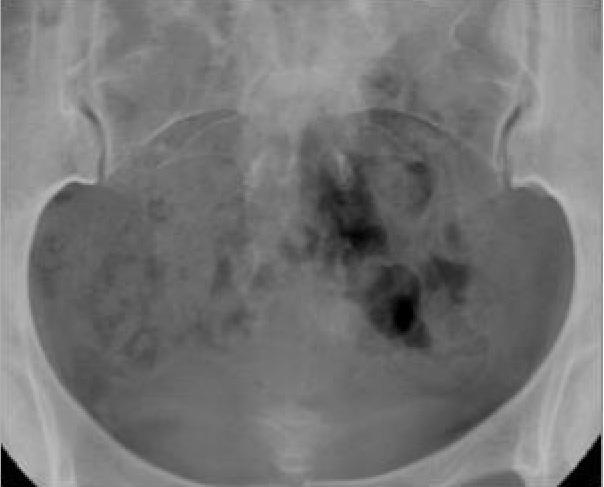
\includegraphics[width=0.5\linewidth]{imagenes/hist1.png}
    \caption{Rx 0 - de pelvis sin contraste}
    \label{fig:h1}
\end{figure}

\begin{figure}
    \centering
    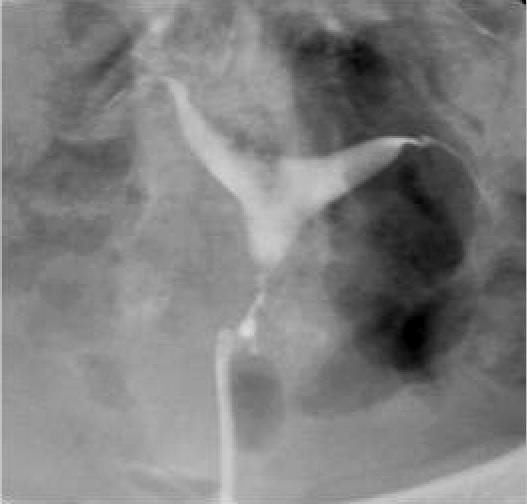
\includegraphics[width=0.5\linewidth]{imagenes/hist2.png}
    \caption{Rx 1 - Llenado precoz}
    \label{fig:h2}
\end{figure}

\begin{figure}
    \centering
    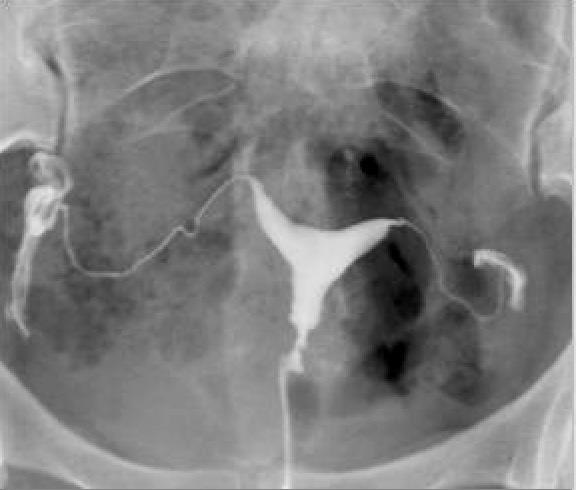
\includegraphics[width=0.5\linewidth]{imagenes/hist3.png}
    \caption{Rx 2 - Cavidad distendida}
    \label{fig:h3}
\end{figure}

\begin{figure}
    \centering
    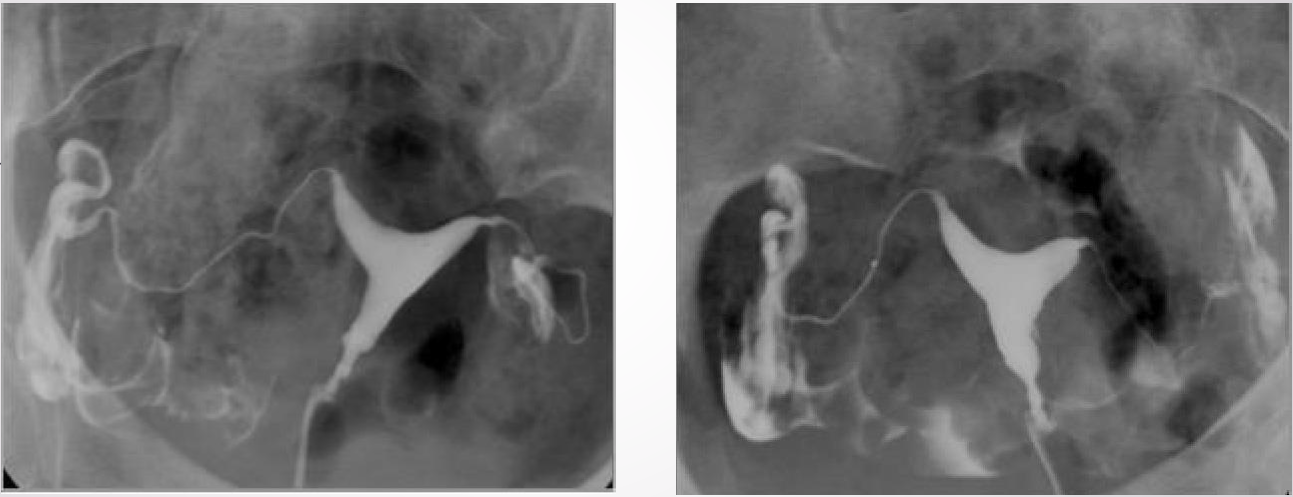
\includegraphics[width=1\linewidth]{imagenes/hist4.png}
    \caption{Rx 3 - Oblicuas}
    \label{fig:h4}
\end{figure}

\begin{figure}
    \centering
    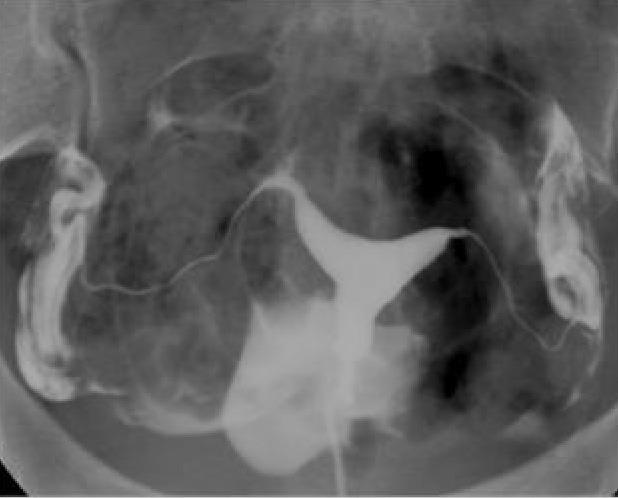
\includegraphics[width=0.5\linewidth]{imagenes/hist5.png}
    \caption{Rx 4 - Paso de MC al peritoneo}
    \label{fig:h5}
\end{figure}

\begin{figure}
    \centering
    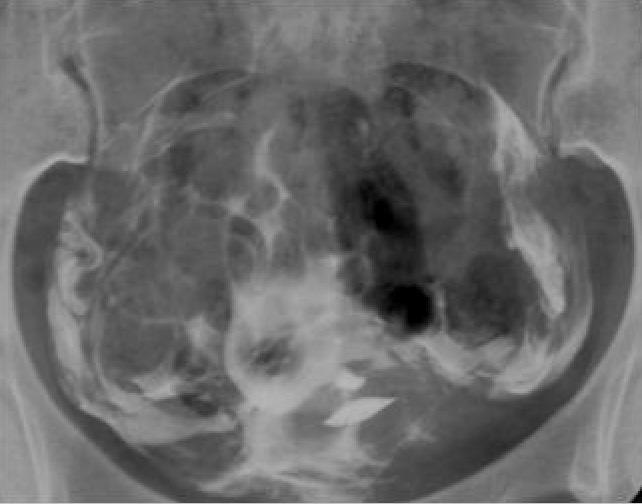
\includegraphics[width=0.5\linewidth]{imagenes/hist6.png}
    \caption{Rx 5 - Post evacuación}
    \label{fig:h6}
\end{figure}

\clearpage

% ============================================================
%  SECCIÓN 7 --- HALLAZGOS PATOLÓGICOS
% ============================================================
\section*{Hallazgos Patológicos Principales}

\subsection*{Espasmo tubárico}

Obstrucción tubárica uni o bilateral que puede afectar a cualquier segmento de la trompa. La etiología más frecuente es la \textbf{infecciosa}. En la HSG se evidencia como ausencia de paso de contraste más allá del sitio de obstrucción.

\begin{figure}[h]
    \centering
    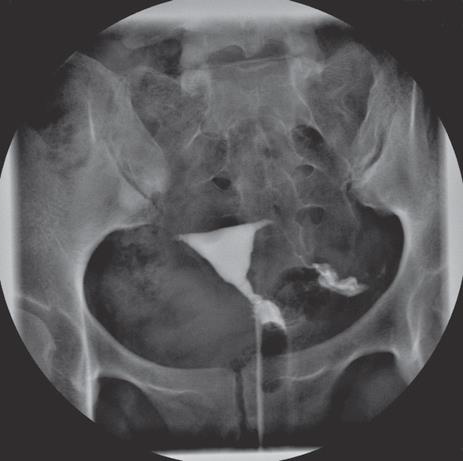
\includegraphics[width=0.5\linewidth]{imagenes/espasmo tubarico.png}
    \caption{Espasmo tubarico}
    \label{fig:h7}
\end{figure}

\subsection*{Malformaciones congénitas uterinas}

Todas derivan de anomalías en el desarrollo o fusión de los \textbf{conductos de Müller (paramesonéfricos)}.

\begin{center}
\begin{tabular}{>{\bfseries}p{2.8cm} p{5.5cm} p{5cm}}
\hline
Malformación & Mecanismo & Aspecto en HSG \\
\hline
Útero unicorne & Ausencia de desarrollo de un conducto de Müller. & Una sola cavidad con una trompa; cavidad y trompa desviadas lateralmente. \\[0.5em]
\hline
Útero didelfo & Falta de fusión completa de los conductos mullerianos. & Dos cavidades uterinas independientes con dos cuellos; requiere cateterización de \textbf{ambos} orificios cervicales. \\[0.5em]
\hline
Útero bicorne & Fusión incompleta de los conductos paramesonéfricos. & Cérvix único con dos cuernos uterinos \textbf{divergentes}; ángulo intercornual \textbf{$>$ 105°}. \\[0.5em]
\hline
Útero septado & Reabsorción incompleta del septo uterovaginal. & Dos cavidades separadas por un septo; ángulo intercornual \textbf{$<$ 75°}. \\
\hline
\end{tabular}
\end{center}

\begin{figure}
    \centering
    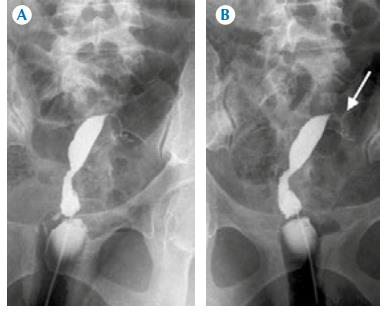
\includegraphics[width=0.5\linewidth]{imagenes/unicorne.png}
    \caption{Útero unicorne}
    \label{fig:h8}
\end{figure}

\begin{figure}
    \centering
    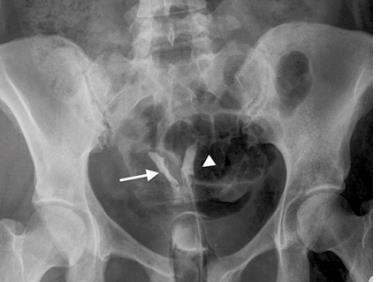
\includegraphics[width=0.5\linewidth]{imagenes/didelfo.png}
    \caption{Útero didelfo}
    \label{fig:h9}
\end{figure}

\begin{figure}
    \centering
    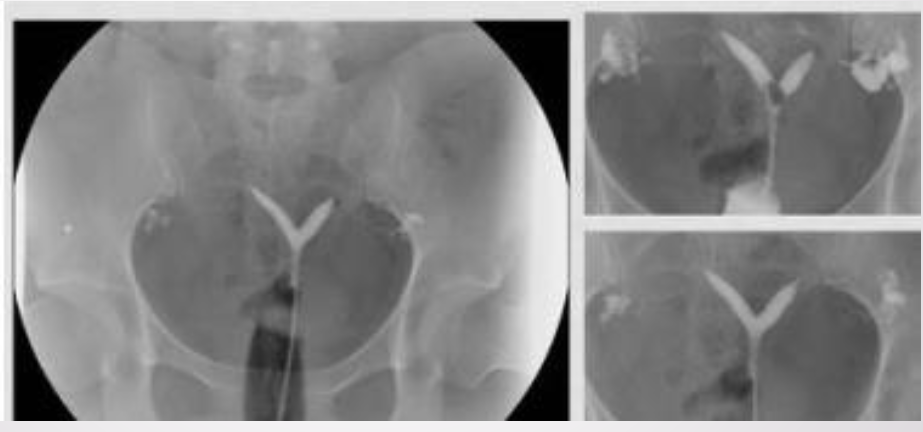
\includegraphics[width=0.5\linewidth]{imagenes/bicorne.png}
    \caption{Útero bicorne}
    \label{fig:h10}
\end{figure}

\begin{figure}
    \centering
    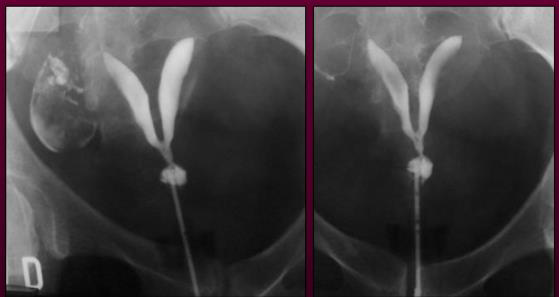
\includegraphics[width=1\linewidth]{imagenes/septado.png}
    \caption{Útero septado}
    \label{fig:h11}
\end{figure}

\clearpage

\begin{cajakeypoints}
\textbf{Diagnóstico diferencial clave:} Bicorne vs. septado se distingue por el \textbf{ángulo intercornual}: $>105°$ = bicorne; $<75°$ = septado.
\end{cajakeypoints}

% ============================================================
%  CIERRE --- ESQUEMA MENTAL FINAL
% ============================================================
\section*{Esquema Mental --- Repaso Final}

\begin{cajakeypoints}
\begin{center}
\textbf{\color{azulprincipal}
  BHCG negativa $\rightarrow$ Fase folicular (día 7--12) $\rightarrow$ Sholkoff 5--7 Fr (istmo) $\rightarrow$ 10 cc contraste $\rightarrow$ Serie de 5 proyecciones}\\[0.4em]
\textbf{\color{naranjadestacado}
  Gold Standard de infertilidad. Permeabilidad confirmada: paso bilateral de contraste a peritoneo.}\\[0.3em]
Balón: jeringa 10 mL de aire \quad Bicorne: $>105°$ \quad Septado: $<75°$ \quad Didelfo: cateterizar ambos cuellos\\[0.3em]
\textbf{Protocolo:} simple $\to$ relleno precoz $\to$ cavidad distendida $\to$ oblicuas $\to$ paso peritoneal $\to$ post-evacuación
\end{center}
\end{cajakeypoints}

\vspace{1em}
\hrule
\vspace{0.5em}

% ============================================================
%  UROLOGÍA INTRAOPERATORIA
%  Licenciatura en Imagenología --- UdelaR
%  Fuente: clase Lic. Matías Prado, Imagenología Especializada I
% ============================================================

\chapter{Urologia Intraoperatoria}


% ============================================================
%  PUNTOS CLAVE PARA EL EXAMEN ORAL
% ============================================================
\begin{cajakeypoints}
\textbf{\color{azulprincipal} Puntos clave para el examen oral}
\begin{itemize}[noitemsep, topsep=2pt]
  \item El licenciado en imagenología es \textbf{personal no estéril}: no puede tocar al cirujano, instrumentista ni la mesa estéril.
  \item \textbf{Catéter Doble J}: acceso retrógrado vía uretra; paciente en decúbito supino con piernas en posición ginecológica (independiente del género).
  \item \textbf{Nefrostomía percutánea}: acceso anterógrado a través de la piel; paciente en decúbito prono; arco en C contralateral al riñón a puncionar.
  \item \textbf{Litotricia endoscópica}: misma posición que Doble J; para cálculos ureterales; sin rayos durante la fragmentación.
  \item \textbf{Litotricia percutánea (nefrolitotomía)}: paciente supino lateralizado con el riñón a trabajar hacia arriba; arco contralateral al riñón afectado.
  \item Los cálculos menores a \textbf{5 mm} se expulsan solos; los mayores a \textbf{8 mm} requieren litotricia percutánea. Entre 5--8 mm: litotricia endoscópica.
  \item Las tres \textbf{estrecheces ureterales} (sitios más frecuentes de cálculos): unión pieloureteral, cruce con vasos ilíacos, y unión ureterovesical.
  \item El contraste utilizado en todos los procedimientos es \textbf{yodado}.
  \item El \textbf{uréter totalmente dilatado} es signo de patología (obstrucción); la ausencia intermitente del uréter en imágenes es normal (peristaltismo).
\end{itemize}
\end{cajakeypoints}

\vspace{1em}

% ============================================================
%  ANATOMÍA DE REFERENCIA	
% ============================================================
\section*{Anatomía de referencia}

\begin{cajadefinicion}
El \textbf{aparato urinario} está constituido por dos riñones, los uréteres, la vejiga y la uretra. Mantiene el equilibrio ácido-base y el balance hidrosalino eliminando desechos metabólicos.
\end{cajadefinicion}

Los riñones son órganos \textbf{retroperitoneales} ubicados entre D12 y L3. El riñón derecho se encuentra más descendido que el izquierdo por la impresión hepática. Anatómicamente no están en el plano sagital: presentan una inclinación de aproximadamente \textbf{20 grados}, lo que tiene implicancia directa en las proyecciones oblicuas durante los procedimientos.
\clearpage

Los uréteres transportan la orina mediante \textbf{ondas peristálticas}. Presentan tres puntos anatómicos de estrechez donde los cálculos se atascan con mayor frecuencia:

\begin{itemize}[noitemsep]
  \item Unión pieloureteral.
  \item Sitio de entrecruzamiento con los vasos ilíacos.
  \item Unión ureterovesical (porción intramural en la cara posterolateral de la vejiga).
\end{itemize}

\subsection*{Personal en block quirúrgico}

El equipo quirúrgico se divide en personal \textbf{estéril} (cirujano, ayudantes, instrumentista: túnica estéril + lavado quirúrgico + guantes) y personal \textbf{no estéril} (licenciado en imagenología, anestesista, auxiliar de enfermería: casaca, pantalón, gorro, tapaboca). El licenciado \textbf{nunca debe tocar} al personal estéril ni la mesa del instrumentista para no contaminar el campo.

% ============================================================
%  CLASIFICACIÓN DE LOS PROCEDIMIENTOS
% ============================================================
\section*{Clasificación de los procedimientos}

\subsection*{Por tipo de acceso y objetivo}

{\renewcommand{\arraystretch}{1.35}
\begin{center}
\begin{tabular}{>{\bfseries}p{3.5cm} p{4.5cm} p{6cm}}
\hline
Procedimiento & Acceso & Objetivo principal \\
\hline
Catéter Doble J & Retrógrado (vía uretra) & Bypass ureteral ante obstrucción o injuria temporal. \\[0.5em]
\hline
Nefrostomía percutánea & Anterógrado (vía piel) & Drenaje externo del riñón obstruido mediante bolsa colectora. \\[0.5em]
\hline
Litotricia endoscópica & Retrógrado (vía uretra) & Fragmentación y extracción de cálculos ureterales ($<$8 mm). \\[0.5em]
\hline
Litotricia percutánea & Anterógrado (vía piel) & Extracción de cálculos renales grandes ($>$8 mm) en pelvis renal. \\
\hline
\end{tabular}
\end{center}

\clearpage

% ============================================================
%  PROCEDIMIENTO 1: CATÉTER DOBLE J
% ============================================================
\section*{Catéter Doble J}

\begin{cajadefinicion}
El \textbf{catéter Doble J} es un tubo fino, flexible y fenestrado que se coloca internamente entre la pelvis renal y la vejiga para asegurar el drenaje de orina ante obstrucciones, lesiones ureterales o como protección posquirúrgica. Sus dos extremos curvados en ``J'' lo fijan en posición. Es un dispositivo \textbf{temporal}.
\end{cajadefinicion}


\subsection*{Indicaciones}
Obstrucción ureteral por cálculo, tumor o estenosis; protección del uréter tras cirugía; tratamiento coadyuvante de litiasis (se deja tras litotricia para favorecer cicatrización de la pared ureteral).

\subsection*{Posición del paciente y distribución de sala}

\begin{itemize}[noitemsep]
  \item Paciente: \textbf{decúbito supino}, piernas en \textbf{posición ginecológica} (independiente del género; el ureteroscopio accede igualmente en ambos sexos).
  \item Cola del paciente pegada al \textbf{borde inferior de la mesa} para permitir que el arco en C llegue hasta el abdomen superior.
  \item Cirujano y ayudante: entre las piernas del paciente.
  \item Instrumentista: a los pies del paciente.
  \item Rack de ureteroscopio: lateral al cirujano.
  \item \textbf{Licenciado en imagenología}: ingresa \textbf{perpendicular}, por el costado que queda libre (opuesto al rack). El monitor de RX se coloca del lado del licenciado.
  \item La entrada del arco en C es \textbf{independiente del riñón} en estudio.\\
\end{itemize}

\begin{cajariesgo}
\textbf{Obstáculos a anticipar:} piernas del paciente, balde debajo de la mesa (el ureteroscopio irriga suero continuamente), base y escalón de la mesa, brazos del paciente, portasueros. Verificar la sala \textbf{antes} de que el paciente esté dormido.
\end{cajariesgo}

\subsection*{Secuencia del procedimiento}

\begin{enumerate}[noitemsep]
  \item El cirujano introduce el \textbf{ureteroscopio} por la uretra hasta la vejiga.
  \item \textbf{Enfoque inicial} del licenciado: frente centrado en vejiga, siguiendo la punta del catéter hasta el meato ureteral.
  \item \textbf{Pielografía retrógrada}: se inyecta contraste yodado a través del catéter recto desde vejiga hacia pelvis renal (sentido contrario a la orina; de ahí el término \textit{retrógrada}). Permite visualizar anatomía, cálculos y estado del uréter.
  \item Se asciende siguiendo la subida del cirujano: el licenciado \textbf{acompaña} el catéter desde vejiga hasta pelvis renal.
  \item Control en pelvis renal: se verifica que la \textbf{guía metálica} esté correctamente posicionada.
  \item Se asciende el \textbf{Doble J} a través de la guía. Se retira la guía; queda solo el catéter.
  \item \textbf{Control final de ambos rulos}: un disparo en pelvis renal (extremo proximal) y un disparo en vejiga (extremo distal). Fin del procedimiento.\\
\end{enumerate}

\begin{cajakeypoints}
\textbf{Concepto clave:} Es el procedimiento urológico más simple y breve ($\sim$10 minutos). No requiere angulaciones especiales ni sustracción digital. Ideal para iniciarse en block quirúrgico.
\end{cajakeypoints}

\begin{figure}[h]
    \centering
    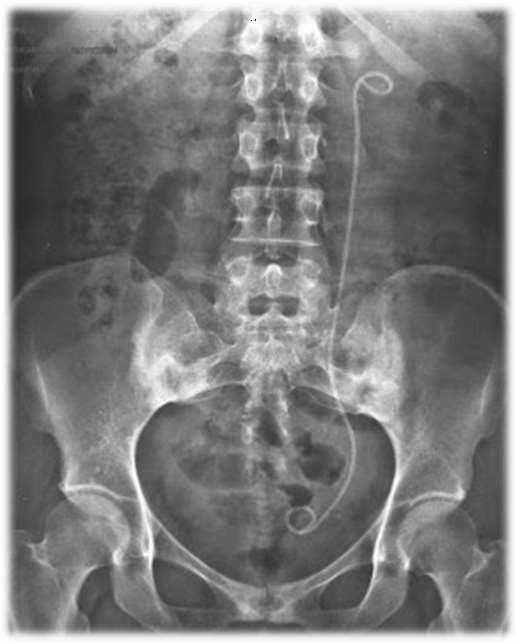
\includegraphics[width=0.5\linewidth]{imagenes/dobleJ.png}
    \caption{Doble J}
    \label{fig:Doble J}
\end{figure}

\clearpage
% ============================================================
%  PROCEDIMIENTO 2: NEFROSTOMÍA PERCUTÁNEA
% ============================================================
\section*{Nefrostomía Percutánea}

\begin{cajadefinicion}
La \textbf{nefrostomía percutánea} consiste en la colocación de un catéter flexible a través de la piel hasta la pelvis renal para drenar orina hacia una bolsa colectora externa. Se indica cuando la obstrucción ureteral no puede resolverse por vía retrógrada o requiere descompresión urgente.
\end{cajadefinicion}

\subsection*{Indicaciones}
Obstrucción ureteral que compromete la función renal, genera dolor o fiebre; preparación previa a litotricia percutánea; obstrucciones no resolubles por vía endoscópica.

\subsection*{Posición del paciente y distribución de sala}

\begin{itemize}[noitemsep]
  \item Paciente: \textbf{decúbito prono} (boca abajo).
  \item Cirujano y ayudantes: del lado del \textbf{riñón a puncionar}.
  \item \textbf{Licenciado en imagenología}: ingresa perpendicular, por el \textbf{lado contralateral} al riñón afectado (lado libre). Si se trabaja el riñón izquierdo, el arco entra por la derecha.
\end{itemize}

\subsection*{Enfoques complementarios}

Los riñones tienen una inclinación de $\sim$20° respecto al plano sagital. Un frente estricto los muestra en oblicua. Para verlos \textbf{de frente} se requiere una oblicua:

{\renewcommand{\arraystretch}{1.35}
\begin{center}
\begin{tabular}{>{\bfseries}p{3cm} p{5.5cm} p{5.5cm}}
\hline
Posición del arco & Técnica & Indicación \\
\hline
PA (boca abajo) & Oblicua \textbf{contralateral}: intensificador se aleja del licenciado, hacia el lado de los médicos. & Visualizar el riñón de frente durante la punción. \\[0.5em]
\hline
AP (hipotético) & Oblicua \textbf{homolateral}: intensificador hacia el licenciado. & Solo orientativo; el procedimiento es siempre en prono. \\
\hline
\end{tabular}
\end{center}
}

\clearpage

\subsection*{Secuencia del procedimiento}

\begin{enumerate}[noitemsep]
  \item \textbf{Enfoque inicial}: frente centrado en el riñón de interés. Referencias anatómicas: columna vertebral (límite medial) y última costilla (límite superior). Riñones entre D12 y L3.
  \item El cirujano realiza la \textbf{punción renal} con aguja de punta abierta. La salida de orina por la punta confirma que está en pelvis renal.

\begin{figure}[h]
    \centering
    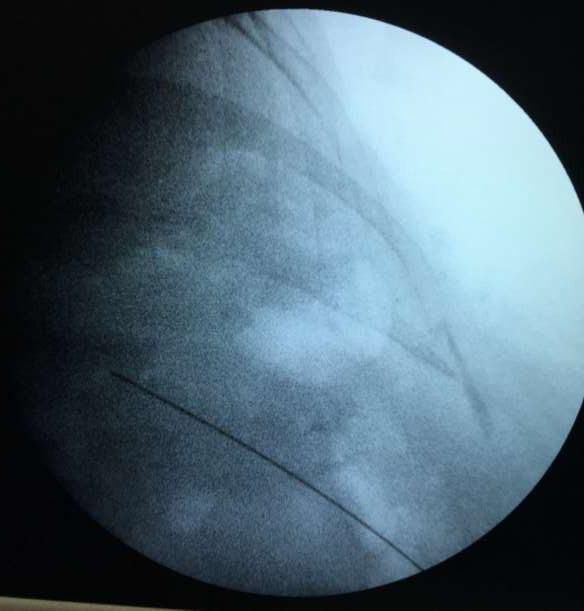
\includegraphics[width=0.5\linewidth]{imagenes/puncionRenal.png}
    \caption{Punción renal}
    \label{fig:puncion}
\end{figure}

  \item \textbf{Pielografía anterógrada}: se inyecta contraste yodado a través de la aguja. Se opacifican cálices, pelvis renal y uréter (sentido de la orina; de ahí \textit{anterógrada}).

\begin{figure}[h]
    \centering
    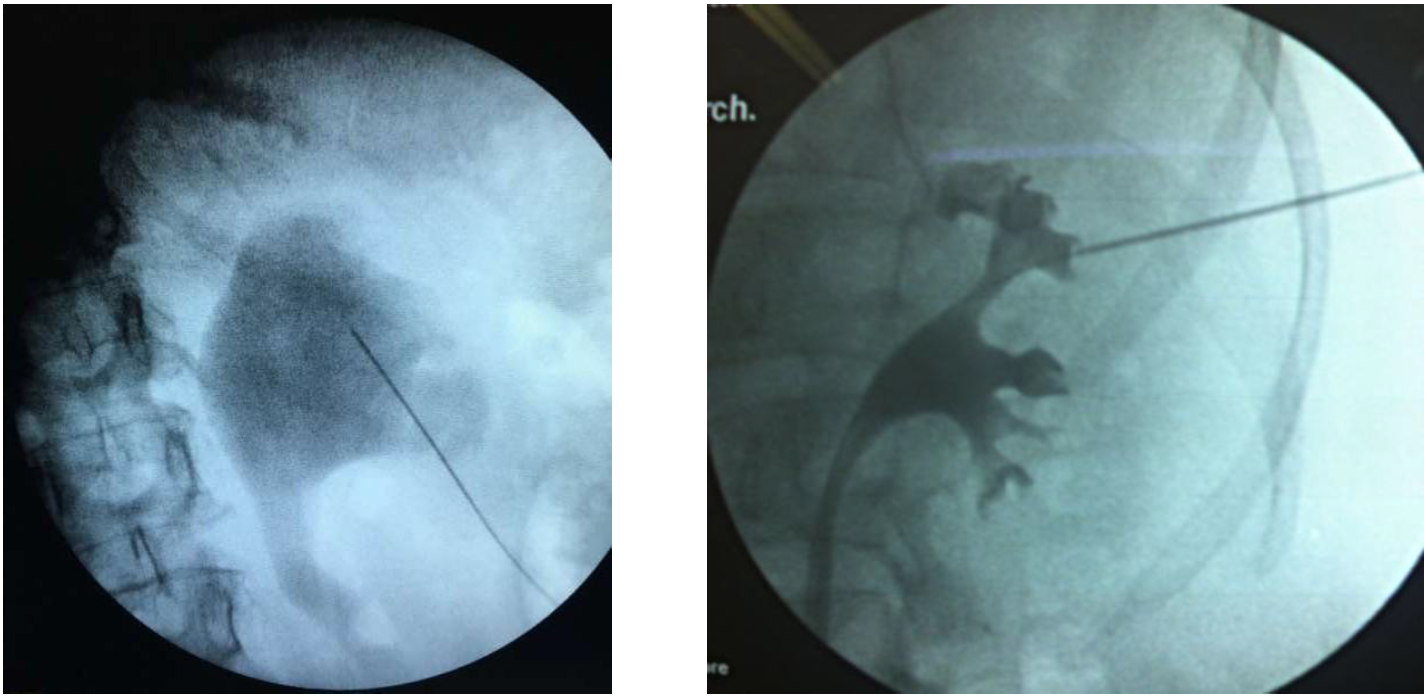
\includegraphics[width=1\linewidth]{imagenes/anterograda.png}
    \caption{Pielografia anterograda}
    \label{fig:pielografia}
\end{figure}

\clearpage


  \item Se pasa la \textbf{guía metálica} a través del catéter de punción.

  \begin{figure}[h]
      \centering
      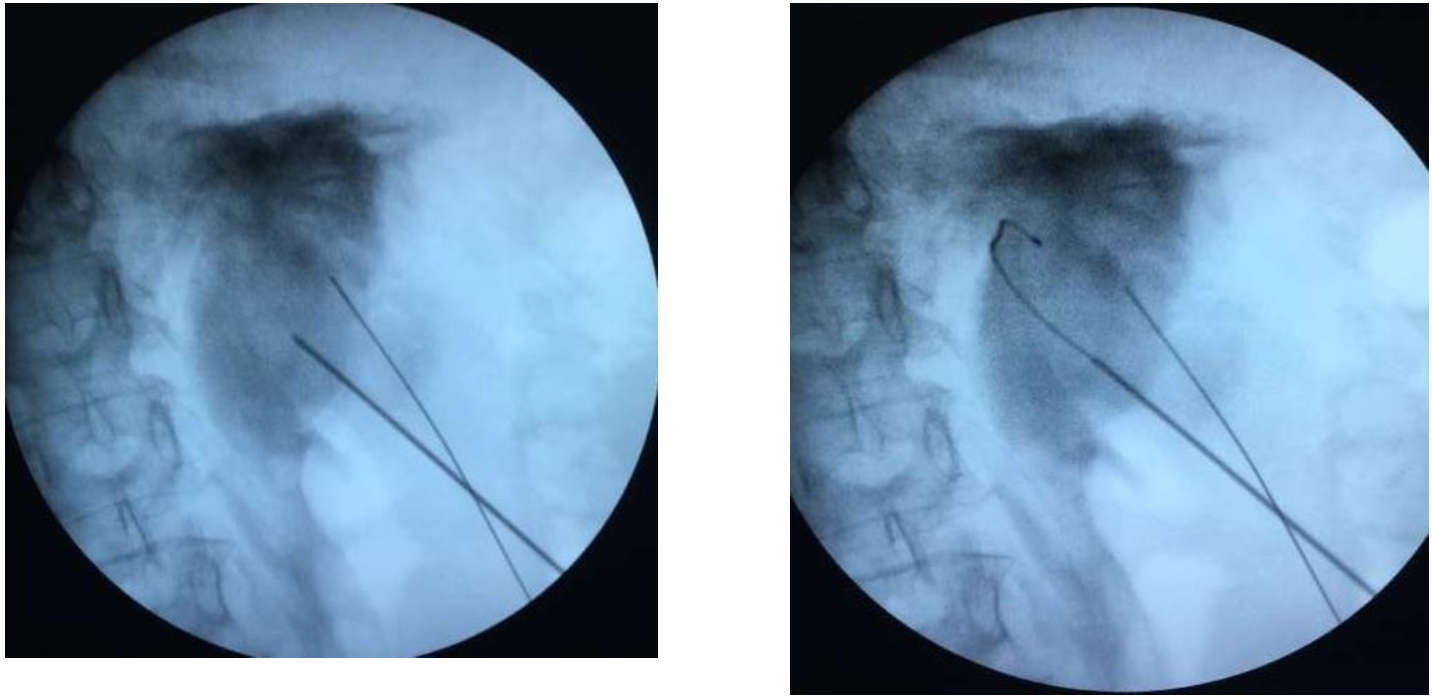
\includegraphics[width=1\linewidth]{imagenes/guia.png}
      \caption{Guía metalica}
      \label{fig:guia}
  \end{figure}

  
  \item Se colocan \textbf{dilatadores} sucesivos sobre la guía para ampliar el trayecto percutáneo.

\begin{figure}[htbp]
    \centering
    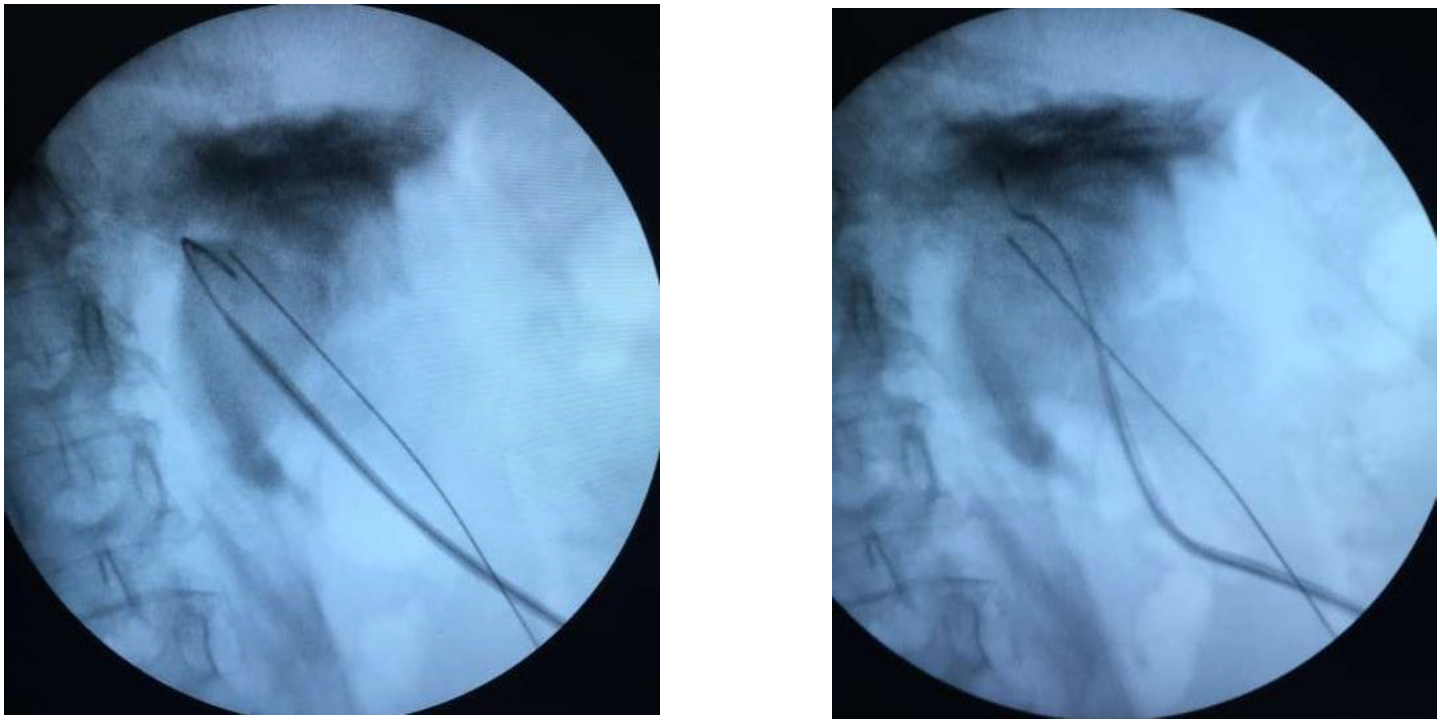
\includegraphics[width=1\linewidth]{imagenes/dilatadores.png}
    \caption{Dilatadores}
    \label{fig:Dilatadores}
\end{figure}
  
  \clearpage
  
  \item Se coloca la \textbf{sonda de nefrostomía} a través de la guía. Se retiran guía y dilatador.
  
  \begin{figure}[htbp]
  	\centering
  	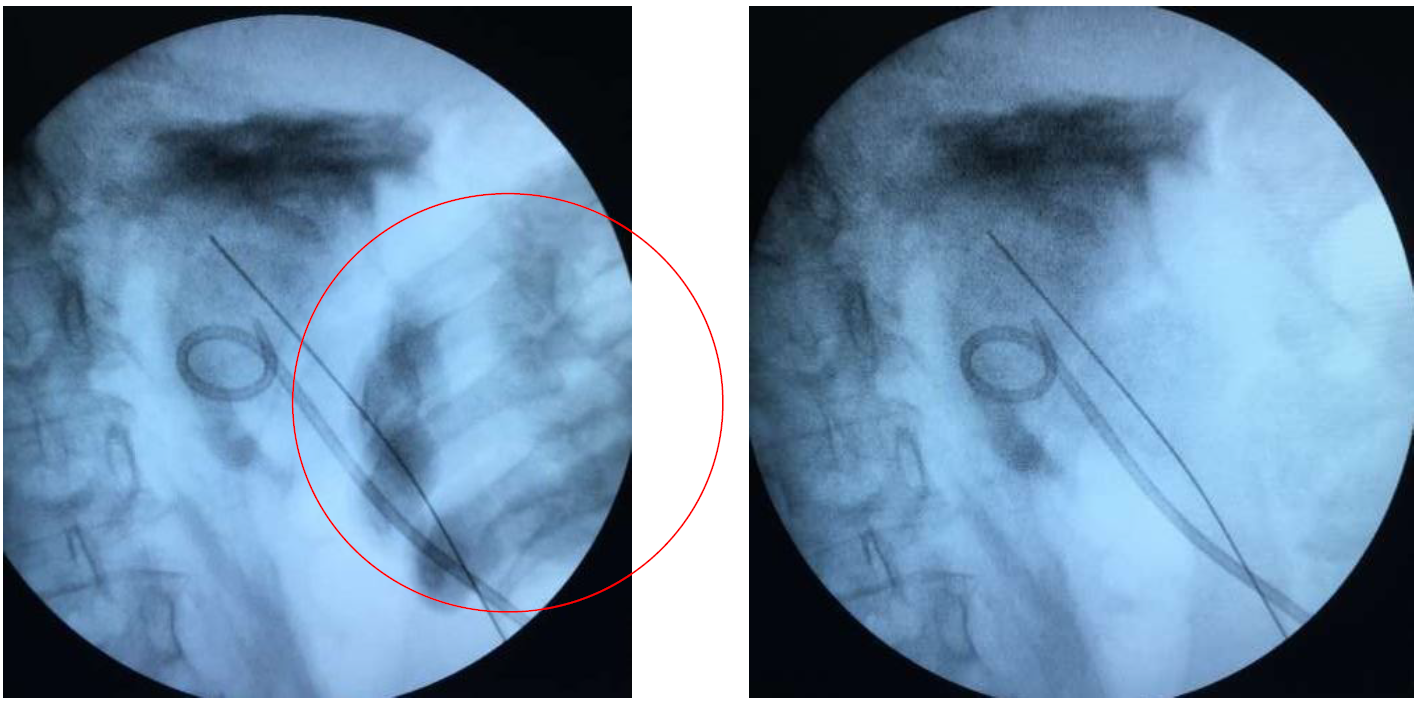
\includegraphics[width=1\linewidth]{screenshot001}
  	\caption{Sonda de nefrostomia}
  	\label{fig:sondanefrostomia}
  \end{figure}
  
  \item \textbf{Pielografía de control final}: se verifica la correcta posición del catéter y la permeabilidad del sistema.
  
\end{enumerate}

  \begin{figure}[h]
	\centering
	\includegraphics[width=0.5\linewidth]{"pielografia final"}
	\caption{Pielografia final}
	\label{fig:pielografia-final}
\end{figure}



\clearpage

\begin{cajariesgo}
\textbf{Importante:} No disparar rayos cuando el cirujano tenga las manos dentro del campo renal. Coordinarse verbalmente antes de cada disparo. El licenciado no se mueve una vez centrado en el riñón; el procedimiento completo se realiza en la misma posición.
\end{cajariesgo}

.\\

\begin{cajakeypoints}
\textbf{Concepto clave:} Radiológicamente es más simple que el Doble J (posición fija durante todo el procedimiento), pero el tiempo total es mayor por la dificultad de la punción percutánea, que puede demandar múltiples intentos del cirujano.
\end{cajakeypoints}

\clearpage
% ============================================================
%  PROCEDIMIENTO 3: LITOTRICIA
% ============================================================
\section*{Litotricia}

\begin{cajadefinicion}
La \textbf{litotricia} es un procedimiento que utiliza ondas de choque para fragmentar cálculos del aparato urinario (riñón, uréter o vejiga) y permitir su eliminación. Solo requieren apoyo radiológico las modalidades \textbf{ureteral} y \textbf{renal}; la vesical se guía exclusivamente por endoscopía.
\end{cajadefinicion}

Estudios previos: ecografía; si no es concluyente, \textbf{Urotac} (TC sin contraste). El 90\% de los cálculos son radiopacos y se visualizan sin contraste. El contraste taparía el cálculo, por lo que se evita en la mayoría de los casos.

\subsection*{Litotricia endoscópica (ureteral)}

\textbf{Indicación:} cálculos ureterales. Posición del paciente y del arco en C: \textbf{idéntica al Doble J} (decúbito supino, piernas en posición ginecológica; licenciado perpendicular por el costado libre).

\begin{enumerate}[noitemsep]
  \item \textbf{Pielografía retrógrada}: igual que en el Doble J. Se localiza el cálculo.
  \item El licenciado acompaña la subida del ureteroscopio \textbf{hasta el cálculo}.
  \item Fragmentación con ondas de choque o láser: \textbf{sin rayos} (el cirujano trabaja por visión endoscópica directa).
  \item Extracción de fragmentos con \textbf{canastilla Dormia} o aspiración.
  \item \textbf{Pielografía de control}: verifica ausencia de cálculos residuales y permeabilidad ureteral.
  \item En la mayoría de los casos se deja un \textbf{Doble J} temporal para proteger el uréter durante la cicatrización (se retira ambulatoriamente en policlínica, sin rayos).
\end{enumerate}

\subsection*{Litotricia percutánea (nefrolitotomía percutánea)}

\textbf{Indicación:} cálculos renales grandes ($>$8 mm) o cuando la vía endoscópica no es viable.

\textbf{Posición del paciente:} \textbf{decúbito supino lateralizado}, con el riñón a trabajar hacia arriba. El licenciado ingresa perpendicular, por el \textbf{lado contralateral} (el que queda abajo). Mismo principio que en nefrostomía percutánea.

\begin{enumerate}[noitemsep]
  \item El cirujano coloca una \textbf{sonda en vejiga} para ocluir el flujo y facilitar el trabajo (no requiere acción del licenciado).
  \item \textbf{Punción renal}: igual que en nefrostomía. El licenciado centra el campo en el riñón y permanece ahí durante todo el procedimiento.
  \item \textbf{Dilatación} del trayecto percutáneo.
  \item Introducción del \textbf{nefroscopio} a través del trayecto dilatado.
  \item Fragmentación de cálculos con ondas de choque.
  \item Extracción de fragmentos.
  \item \textbf{Pielografía anterógrada final}: verifica limpieza de la pelvis renal.
  \item Se deja un \textbf{set de nefrostomía} temporal para el período de recuperación.
\end{enumerate}

\clearpage

\begin{cajakeypoints}
\textbf{Proyección de perfil (complementaria):} Girar el arco en C a 90° a pedido del cirujano. El perfil informa la \textbf{altura de trabajo} del arco; establecida esa altura, mantenerla fija para todo el procedimiento (tanto en frente como en perfil). Avisar al cirujano antes de girar el arco para que se retire del campo.
\end{cajakeypoints}

.\\


\begin{cajariesgo}
\textbf{Posición correcta del paciente:} La zona de trabajo (pelvis renal) debe quedar libre hacia arriba y hacia abajo para poder realizar tanto el frente como el perfil. Si el paciente no está bien posicionado, corregirlo \textbf{antes} de iniciar el procedimiento. No tener vergüenza en solicitarlo: el resto del equipo no sabe lo que el licenciado necesita mostrar.
\end{cajariesgo}

% ============================================================
%  TABLA COMPARATIVA DE LOS CUATRO PROCEDIMIENTOS
% ============================================================
\section*{Tabla comparativa de los procedimientos}

{\renewcommand{\arraystretch}{1.35}
	\begin{center}
		\begin{tabular}{>{\bfseries}p{3cm} >{\centering}p{2.8cm} >{\centering}p{2.8cm} >{\centering}p{2.8cm} >{\centering\arraybackslash}p{2.8cm}}
			\hline
			\textbf{Criterio} & \textbf{Doble J} & \textbf{Nefrostomía} & \textbf{Litotricia endosc.} & \textbf{Litotricia percutánea} \\
			\hline
			Posición paciente & Supino + ginecológica & Decúbito prono & Supino + ginecológica & Supino lateralizado \\[0.5em]
			\hline
			Acceso & Retrógrado (uretra) & Anterógrado (piel) & Retrógrado (uretra) & Anterógrado (piel) \\[0.5em]
			\hline
			Lado del licenciado & Costado libre (cualquiera) & Contralateral al riñón & Costado libre (cualquiera) & Contralateral al riñón \\[0.5em]
			\hline
			Pielografía & Retrógrada & Anterógrada & Retrógrada + control final & Anterógrada final \\[0.5em]
			\hline
			Duración aprox. & $\sim$10 min & 30--60 min & 20--40 min & 60--90 min \\[0.5em]
			\hline
			Complejidad Lic. & Baja & Muy baja (posición fija) & Baja & Baja (posición fija) \\
			\hline
		\end{tabular}
	\end{center}
}

\clearpage
% ============================================================
%  ESQUEMA MENTAL --- REPASO FINAL
% ============================================================
\section*{Esquema Mental --- Repaso Final}

\begin{cajakeypoints}
\begin{center}
\textbf{\color{azulprincipal}
  Obstrucción ureteral $\rightarrow$ elegir vía $\rightarrow$ retrógrada (endoscópica) o anterógrada (percutánea)}\\[0.4em]
\textbf{\color{naranjadestacado}
  Si el paciente está boca arriba con piernas en posición ginecológica: entro por el costado libre. Si está boca abajo o lateralizado: entro por el lado contralateral al riñón afectado.}\\[0.3em]
Cálculo $<5$ mm: expulsión espontánea \quad $5$--$8$ mm: litotricia endoscópica \quad $>8$ mm: litotricia percutánea\\[0.3em]
90\% de cálculos son radiopacos $\to$ Urotac sin contraste \quad Contraste utilizado: yodado\\[0.3em]
\textbf{Doble J:} cateterismo $\to$ pielografía retrógrada $\to$ guía metálica $\to$ ascenso DJ $\to$ control ambos rulos\\[0.2em]
\textbf{Nefrostomía:} punción renal $\to$ pielografía anterógrada $\to$ guía $\to$ dilatadores $\to$ catéter $\to$ pielografía final\\[0.2em]
\textbf{Litotricia endosc.:} igual que DJ hasta cálculo $\to$ ondas (sin rayos) $\to$ extracción $\to$ pielografía control $\to$ DJ\\[0.2em]
\textbf{Litotricia percutánea:} sonda vejiga $\to$ punción $\to$ dilatación $\to$ nefroscopio $\to$ fragmentación $\to$ extracción $\to$ pielografía anterógrada $\to$ nefrostomía\\
\end{center}
\end{cajakeypoints}

\vspace{1em}
\hrule
\vspace{0.5em}
{\footnotesize \textit{Fuente: material de clase --- Doc. Asis. Lic. Matías Prado,
  Imagenología Especializada I, UdelaR 2026.}}
% ============================================================
%  ESTUDIOS CONTRASTADOS DIGESTIVOS
%  Licenciatura en Imagenología --- UdelaR
%  Dr. Nicolás Asteggiante -- Asis. Lic. Gonzalo Ferreira
%  Unidad Académica de Imagenología, 2026
% ============================================================

\chapter{Estudios contrastados digestivos}



% ============================================================
%  PUNTOS CLAVE PARA EL EXAMEN ORAL
% ============================================================
\begin{cajakeypoints}
	\textbf{\color{azulprincipal} Puntos clave para el examen oral}
	\begin{itemize}[noitemsep, topsep=2pt]
		\item Un estudio contrastado modifica la \textbf{densidad} del órgano mediante un fármaco (medio de contraste) y radiaciones ionizantes; tiene utilidad \textbf{anatómica y funcional}.
		\item Contrastes \textbf{positivos}: sulfato de bario (Z=56) y yodado hidrosoluble (Z=53). Contrastes \textbf{negativos}: aire, sales efervescentes. El \textbf{doble contraste} combina ambos.
		\item El bario se usa en estudios de rutina; el \textbf{yodado hidrosoluble} es obligatorio cuando se sospecha \textbf{perforación, fuga o fístula} (el bario en mediastino/peritoneo causa reacción inflamatoria grave).
		\item El \textbf{estudio de la deglución} evalúa disfagia orgánica o funcional; se inicia siempre con consistencia \textbf{semisólida} para evitar aspiración.
		\item En el \textbf{EGD} la posición de elección es la \textbf{OAD} (oblicua anterior derecha) para despejar el esófago de la columna. El paciente debe estar en \textbf{ayunas 6 horas} y no fumar/mascar chicle.
		\item El \textbf{colon por enema} se realiza con bario + aire (doble contraste); requiere preparación con laxante el día previo y cánula por vía anal en decúbito prono.
		\item La \textbf{colangiografía postoperatoria} usa contraste yodado diluido al 50\% inyectado por el tubo de Kehr; evalúa litiasis residual, estenosis y permeabilidad al duodeno.
		\item Signo patognomónico de \textbf{acalasia}: ``punta de lápiz'' o ``cola de ratón''. Signo de estenosis neoplásica: bordes ``en corazón de manzana'', rigidez segmentaria, defecto de llenado.
	\end{itemize}
\end{cajakeypoints}

\vspace{1em}

% ============================================================
%  SECCIÓN 1 --- DEFINICIÓN
% ============================================================
\section*{Definición}

\begin{cajadefinicion}
	Un \textbf{estudio contrastado} es un procedimiento médico que utiliza \textbf{radiaciones ionizantes} y la administración de un \textbf{medio de contraste} (fármaco de alto número atómico) para visualizar estructuras que, por sí solas, son indistinguibles de su entorno por tener densidad similar a los tejidos adyacentes.
\end{cajadefinicion}

Su objetivo es cambiar la densidad de órganos huecos (como esófago, estómago, colon o vía biliar) permitiendo su diferenciación en radiología convencional. Son estudios complementarios, solicitados habitualmente por el cirujano en contexto postoperatorio o por el gastroenterólogo. Su utilidad es \textbf{doble}: anatómica (forma, estructura, calibre) y funcional (motilidad, tránsito, competencia de esfínteres).

% ============================================================
%  SECCIÓN 2 --- CLASIFICACIÓN DE MEDIOS DE CONTRASTE
% ============================================================
\section*{Clasificación de los Medios de Contraste}

\subsection*{Contrastes positivos (aumentan densidad)}

{\renewcommand{\arraystretch}{1.35}
	\begin{center}
		\begin{tabular}{>{\bfseries}p{3.5cm} p{5.5cm} p{4.5cm}}
			\hline
			Contraste & Características & Uso principal \\
			\hline
			Sulfato de bario & Sal mineral inerte, viscosa; no se absorbe; se elimina por vía rectal. Se adhiere a la mucosa (\textit{mucosografía}). & Estudios de rutina del tubo digestivo: EGD, colon por enema, tránsito del delgado. \\[0.5em]
			\hline
			Yodado hidrosoluble & No iónico, baja osmolaridad (ej. Omnipaque, Z=53). No se adhiere a la mucosa. & Postoperatorios, sospecha de perforación/fuga/fístula, colangiografía, prequirúrgico de reconstrucción. \\
			\hline
		\end{tabular}
	\end{center}
}
.\\
\begin{cajakeypoints}
	\textbf{Regla de oro:} Si hay sospecha de que el contraste puede salir del tubo digestivo (perforación, anastomosis reciente, fístula), usar \textbf{siempre yodado hidrosoluble}. El bario libre en mediastino o peritoneo produce \textbf{mediastinitis o peritonitis química} de manejo muy difícil.
\end{cajakeypoints}

\subsection*{Contrastes negativos (disminuyen densidad)}

Se utilizan para distender el órgano y generar contraste mediante gas. En el \textbf{colon por enema} se usa \textbf{aire}; en el \textbf{EGD} se utilizan \textbf{sales efervescentes} (bicarbonato de sodio, carbonato de sodio, ácido cítrico; marca comercial tipo Uvasal). La combinación de un contraste positivo con uno negativo produce el \textbf{doble contraste}: el gas distiende la luz y el bario pinta la mucosa, permitiendo ver el detalle fino de los pliegues.

% ============================================================
%  SECCIÓN 3 --- ESTUDIOS DEL TUBO DIGESTIVO
% ============================================================
\section*{Estudios del Tubo Digestivo}

\subsection*{Estudio de la Deglución}

Evalúa la \textbf{disfagia} (dificultad para tragar), que puede ser \textbf{orgánica} (causa estructural: tumor, divertículo de Zenker, lesión cáustica, osteofitos) o \textbf{funcional} (causa neuromuscular: ACV, ELA, Alzheimer, miastenia gravis). Es un estudio \textbf{dinámico} realizado bajo \textbf{radioscopia en tiempo real}.

\textbf{Preparación:} Paciente en ayunas. Si tiene SNG, retirarla 12 horas antes.

\textbf{Materiales -- protocolo artesanal} (sulfato de bario en tres consistencias):
\begin{itemize}[noitemsep]
	\item \textbf{Líquida:} SB 170 mg en 100 cc de agua.
	\item \textbf{Semisólida:} SB 170 mg en 50 cc de agua + 5 mg de espesante.
	\item \textbf{Sólida:} Trozo de pan de 5 g sumergido en SB.
\end{itemize}

\textbf{Orden de administración (crítico para seguridad):} Siempre comenzar por la \textbf{consistencia semisólida}. Iniciar con líquido podría causar una aspiración masiva que impediría completar el estudio.

\textbf{Técnica:} El paciente realiza un buche sin tragar; bajo radioscopia el médico da la orden de deglutir y se captura una secuencia de disparos seriada (video) en \textbf{perfil} (tiempos de deglución) y \textbf{frente} (residuos en valéculas y senos piriformes). En un estudio normal no debe quedar residuo en estos sectores.

\textbf{Hallazgos críticos:}
\begin{itemize}[noitemsep]
	\item \textbf{Penetración:} el contraste entra al vestíbulo laríngeo pero se detiene en las cuerdas vocales.
	\item \textbf{Aspiración:} el contraste sobrepasa la glotis; se visualizan tráquea y bronquios ``pintados'' de bario.
\end{itemize}

\textbf{Rol del Licenciado:} Adquirir la secuencia de video completa. El médico asiste al paciente (frecuentemente en silla de ruedas o con movilidad reducida) mientras el licenciado opera el equipo.

% ---
\subsection*{Esofagogastroduodeno (EGD / SEGD)}

Evaluación anatómica y funcional del esófago, estómago y duodeno mediante doble contraste. Indicaciones principales: disfagia funcional u orgánica, ERGE, hernia hiatal, estenosis, postoperatorio de cirugías esofágicas o gástricas (cirugías de Nissen, bariátricas).

\textbf{Preparación:} Ayuno mínimo de 6 horas. No fumar, mascar chicle, ni tomar mate (producen saliva y gas que arruinan la adherencia del bario). No se usa Buscapina (para conservar la evaluación de la motilidad).

\textbf{Materiales:} Sales efervescentes disueltas en poca agua (el paciente las bebe rápido sin eructar) + bario diluido. Aproximadamente \textbf{5 chasis 35$\times$43}, apaisados y verticales según la fase.

\textbf{Parámetros técnicos:} Alto kVp (escala larga de grises para compensar el contraste del bario) y tiempos de exposición cortos (evitar borrosidad por peristaltismo). Referencia: 70 kV / 10--20 mAs según el sector.

\clearpage

\textbf{Secuencia de posiciones y fases:}

{\renewcommand{\arraystretch}{1.35}
	\begin{center}
		\begin{tabular}{>{\bfseries}p{3.5cm} p{5cm} p{5cm}}
			\hline
			\textbf{Posición} & \textbf{Dinámica del contraste} & \textbf{Objetivo} \\
			\hline
			Bipedestación perfil & Buche de bario diluido; evaluación dinámica de la faringe. & Descartar aspiración antes de proceder. \\[0.5em]
			\hline
			Bipedestación OAD & Paciente apoya hombro izquierdo, eleva lado derecho. & Despejar esófago de columna y corazón; esófago en repleción y doble contraste. \\[0.5em]
			\hline
			Bipedestación frente & Rayo horizontal. Nivel hidroaéreo visible. & Fundus en doble contraste (aire); cuerpo y antropíloro en repleción por gravedad. \\[0.5em]
			\hline
			Decúbito supino frente & Bario se desplaza a zonas posteriores. & Fundus y antro distal en repleción; cuerpo gástrico en doble contraste (anterior). \\[0.5em]
			\hline
			Decúbito OAD & Paciente gira hacia su izquierda. & Fundus en repleción; cuerpo y antropíloro en doble contraste. \\[0.5em]
			\hline
			Decúbito OAI + maniobras reflujo & Paciente gira hacia su derecha; Trendelenburg; deglución de saliva. & Fundus, antropíloro y bulbo en repleción; evaluación del esfínter esofágico inferior. \\[0.5em]
			\hline
			Decúbito prono / OPI & Casi boca abajo; bario pasa al duodeno por gravedad. & Documentar las 4 porciones del duodeno (bulbo, descendente, horizontal, ascendente). \\[0.5em]
			\hline
			Decúbito OAD final & Se vuelve a OAD tras movilizar al paciente. & Duodeno en doble contraste (la posición más difícil de lograr). \\
			\hline
		\end{tabular}
	\end{center}
}

\begin{cajakeypoints}
	\textbf{Anatomía del duodeno:} Bulbo (1\textordfeminine\ porción): liso, sin estriaciones. Porciones 2, 3 y 4: pliegues circulares. La 2\textordfeminine\ porción recibe los conductos biliar y pancreático. La 4\textordfeminine\ finaliza en el \textbf{ángulo de Treitz}.
\end{cajakeypoints}

\textbf{Maniobras de mesa:}
\begin{itemize}[noitemsep]
	\item \textbf{Trendelenburg} (cabeza abajo): rellena sectores superiores con bario; fuerza el reflujo gastroesofágico.
	\item \textbf{Anti-Trendelenburg} (cabeza arriba): desplaza bario hacia sectores inferiores; útil para doble contraste superior.
\end{itemize}


\textbf{Postoperatorio urgente:} Si hay sospecha de fuga antes del alta, usar \textbf{yodado hidrosoluble diluido} en lugar de bario. Control estándar postquirúrgico: a los 3 meses.

\clearpage
% ---
\subsection*{Tránsito Esofágico (postoperatorio de esofagectomía)}

Se indica específicamente para control tras \textbf{esofagectomía con ascenso gástrico} (resección de esófago por cáncer y reconstrucción con estómago). El punto crítico es la \textbf{anastomosis}. Se utiliza \textbf{yodado hidrosoluble} (riesgo de fuga al mediastino).

\textbf{Proyecciones obligatorias:} frente estricto, OAD, OAI y \textbf{perfil} (para detectar fugas anteriores o posteriores). Chasis 35$\times$43 apaisado dividido en dos. El órgano reconstruido suele verse dilatado o tortuoso: hallazgo esperable.

\textbf{Protocolo en disfagia progresiva grave:}
\begin{enumerate}[noitemsep]
	\item Iniciar con buche de yodado hidrosoluble bajo radioscopia.
	\item Si no hay fuga ni paso a la vía aérea, proceder con bario.
	\item En estenosis muy severa, \textbf{no administrar sales efervescentes} (riesgo de rotura esofágica por distensión brusca).
\end{enumerate}

% ---
\subsection*{Tránsito del Intestino Delgado}

Consiste en administrar bario oral y documentar su avance por yeyuno e íleon mediante \textbf{radiografías seriadas cada 30--60 minutos}, hasta opacificar el \textbf{ciego} (válvula ileocecal). Es de bajo rendimiento diagnóstico actual; ha sido ampliamente desplazado por la \textbf{enterotomografía} y la \textbf{enterorresonancia}. Aún se utiliza en postoperatorios para evaluar reactivación del tránsito (\textbf{íleo paralítico}).

% ---
\subsection*{Colon por Enema}

Alternativa a la videocolonoscopía (VCC) cuando esta es incompleta por estenosis o colon flexuoso, o en jóvenes con estreñimiento crónico (sospecha de dolicocolon / megacolon). También se usa en el prequirúrgico de reconstrucción de colostomías (ambos cabos con yodado).

\textbf{Preparación:} Dieta + laxantes desde el día anterior (colon libre de materia fecal).

\textbf{Preparación del contraste:} Bario en polvo disuelto en 800 cc -- 1,5 litros de agua tibia; se bate, se presuriza con perita y se clampea la bolsa.

\textbf{Secuencia del estudio:}
\begin{enumerate}[noitemsep]
	\item Paciente en \textbf{decúbito prono}; se introduce cánula por el ano.
	\item \textbf{Fase de llenado:} la bolsa colgada permite entrada de bario por gravedad bajo control radioscopio; cuando llega al colon transverso medio, se baja al piso (maniobra de retorno) para que el exceso regrese a la bolsa dejando la mucosa ``pintada'' hasta el colon derecho.
	\item \textbf{Fase de doble contraste:} se inyecta aire pisando la bolsa manualmente; el aire distiende el colon y el bario adherido revela el relieve mucoso.
	\item \textbf{Documentación:} rotación artesanal del paciente bajo radioscopia para desplegar los \textbf{ángulos hepático y esplénico}. Proyecciones obligatorias: decúbito supino frente, ambas oblicuas, \textbf{perfil de recto} (ampolla rectal y espacio presacro) y \textbf{bipedestación} (niveles hidroaéreos y movilidad).
\end{enumerate}

\textbf{Chasis:} Aproximadamente 5 chasis 35$\times$43 (la mayoría divididos en dos exposiciones).

\textbf{Rol del Licenciado:} Si el médico está a pie de tubo rotando al paciente, el licenciado dispara, centra y cambia chasis rápidamente. Es un estudio artesanal y médico-dependiente.\\

\begin{cajakeypoints}
	\textbf{Principio ``menos es más'':} Usar volumen moderado de bario. Exceso de bario en el colon tapa la mucosa y dificulta ver pólipos o lesiones (imágenes muy blancas con superposición). El Licenciado debe estar con \textbf{chaleco plomado} durante la fase de aire porque opera la bolsa a pie de tubo.
\end{cajakeypoints}

% ============================================================
%  SECCIÓN 4 --- ESTUDIOS DE GLÁNDULAS ANEXAS
% ============================================================
\section*{Estudios de Glándulas Anexas}

\subsection*{Colangiografía Postoperatoria (Tubo en T / Tubo de Kehr)}

Se realiza en el postoperatorio de \textbf{colecistectomía} para evaluar litiasis residual, estenosis postquirúrgica y permeabilidad del contraste al duodeno. Aunque la \textbf{colangiorresonancia} es la técnica de elección actual, este estudio sigue vigente por accesibilidad.

\textbf{Material:} Tubo de Kehr (tubo en T dejado por el cirujano en el colédoco o conducto cístico). Contraste \textbf{yodado hidrosoluble diluido al 50\%} con solución fisiológica (para no tapar pequeños cálculos con una densidad excesiva).

\textbf{Técnica:} Inyección muy lenta y constante con jeringa de 10 cc (evitar espasmos y burbujas de aire, que se confunden con cálculos). Se busca opacificar toda la vía biliar intra y extrahepática.

\textbf{Proyecciones:} Frente en decúbito dorsal + oblicua anterior izquierda (OAI) para desplegar los conductos hepáticos de la columna. Chasis 35$\times$43 dividido en dos.

\textbf{Criterios de evaluación:}
\begin{itemize}[noitemsep]
	\item Ausencia de defectos de relleno (cálculos residuales).
	\item Llenado completo de los conductos hepáticos derecho e izquierdo.
	\item Paso libre del contraste al \textbf{duodeno} (esfínter de Oddi permeable).
\end{itemize}

\subsection*{Sialografía}

Estudio de las glándulas salivales mayores (parótida y submaxilar) para evaluar anatomía de conductos excretores y detectar \textbf{sialolitiasis}. Ha perdido terreno frente a la resonancia, pero persiste para detección de cálculos.

\textbf{Técnica artesanal:}
\begin{enumerate}[noitemsep]
	\item Estimular la secreción con \textbf{jugo de limón} para identificar el orificio ductal.
	\item Cateterizar con \textbf{aguja roma} (sin punta).
	\item Inyectar contraste \textbf{yodado hidrosoluble}.
\end{enumerate}

\textbf{Conductos y localización:}
\begin{itemize}[noitemsep]
	\item \textbf{Conducto de Stenon (parótida):} orificio a nivel del 2\textordfeminine/3\textsuperscript{er} molar superior.
	\item \textbf{Conducto de Wharton (submaxilar):} orificio en el piso de la boca, detrás de la arcada dentaria inferior (carúncula sublingual).
\end{itemize}

\textbf{Proyecciones:} AP y lateral sin contraste (base), luego fase de llenado y fase de vaciado (perfil y oblicuas de mandíbula ``desenfilado'').

% ============================================================
%  SECCIÓN 5 --- HALLAZGOS PATOLÓGICOS RELEVANTES
% ============================================================
\section*{Hallazgos Patológicos Relevantes}

\subsection*{Signos radiológicos: Esófago}

{\renewcommand{\arraystretch}{1.3}
	\begin{center}
		\begin{tabular}{>{\bfseries}p{3.5cm} p{5cm} p{5cm}}
			\hline
			\textbf{Patología} & \textbf{Signos radiológicos} & \textbf{Clínica / Nota} \\
			\hline
			Divertículo de Zenker & Imagen de adición redondeada u ovalada en pared posterior cervical (triángulo de Killian); se rellena de bario antes que el esófago distal. Confirmar en \textbf{perfil estricto}. & Disfagia alta, regurgitación, halitosis. Riesgo: perforación endoscópica si no se detecta antes. \\[0.5em]
			\hline
			Estenosis neoplásica & Defecto de llenado, bordes ``mordidos'' o ``en corazón de manzana'', rigidez segmentaria (sin ondas peristálticas), dilatación suprastenótica + nivel hidroaéreo. & Disfagia progresiva: sólidos $\to$ líquidos $\to$ afagia. \\[0.5em]
			\hline
			Acalasia & ``Punta de lápiz'' / ``cola de ratón'' (signo patognomónico): estrechamiento suave y simétrico en la unión esofagogástrica. Megaesófago / esófago sigmoideo. Ausencia de burbuja gástrica. & Trastorno funcional; esfínter esofágico inferior no se relaja. DD con cáncer: bordes lisos (acalasia) vs. bordes irregulares (neoplasia). \\
			\hline
		\end{tabular}
	\end{center}
}

\subsection*{Signos radiológicos: Estómago}

\textbf{Úlcera gástrica:} El bario rellena el cráter generando una \textbf{imagen de adición} que sobresale del contorno gástrico. Sitio más frecuente: \textbf{curvatura menor}. Benignidad: nicho liso y redondeado con pliegues que convergen simétricamente. Malignidad: nicho dentro de una masa, bordes irregulares, no sobrepasa la línea de la pared.

\textbf{Neoplasia gástrica:} Interfase abrupta e irregular, rigidez segmentaria (zona fija, ``congelada'', sin peristaltismo), defecto de llenado asimétrico.

% ============================================================
%  SECCIÓN 6 --- RADIOPROTECCIÓN
% ============================================================
\section*{Radioprotección en Estudios Contrastados}

Estos estudios implican uso de radiaciones ionizantes. Los efectos biológicos son:
\begin{itemize}[noitemsep]
	\item \textbf{Estocásticos:} aleatorios, proporcionales a la dosis acumulada (ej. riesgo de cáncer).
	\item \textbf{Determinísticos:} aparecen tras superar un umbral de dosis (ej. radiodermitis).
\end{itemize}

\textbf{Principio ALARA:} obtener la mayor calidad de imagen con la menor exposición posible.

\textbf{EPP obligatorio} (el personal suele estar a pie de tubo durante el estudio):

{\renewcommand{\arraystretch}{1.25}
	\begin{center}
		\begin{tabular}{>{\bfseries}p{4cm} p{9cm}}
			\hline
			Elemento & Protege \\
			\hline
			Chaleco plomado & Torso (órganos radiosensibles: tiroides, gónadas, médula ósea). \\
			\hline
			Protector de tiroides & Glándula tiroidea (muy radiosensible). \\
			\hline
			Lentes plomados & Cristalino (riesgo de catarata por dosis acumulada). \\
			\hline
		\end{tabular}
	\end{center}
}
.\\

\begin{cajariesgo}
	\textbf{Importante:} El uso de \textbf{radioscopia} debe minimizarse al máximo (solo para centrar y controlar el paso del contraste). La documentación diagnóstica se realiza con la \textbf{exposición radiográfica en el momento justo}. En el colon por enema, el Licenciado opera la bolsa de aire \textbf{a pie de tubo}: el chaleco es indispensable.
\end{cajariesgo}

% ============================================================
%  ESQUEMA MENTAL --- REPASO FINAL
% ============================================================
\section*{Esquema Mental --- Repaso Final}

\begin{cajakeypoints}
	\begin{center}
		\textbf{\color{azulprincipal}
			Alto Z $\rightarrow$ Efecto fotoeléctrico $\rightarrow$ Mayor densidad en imagen $\rightarrow$ Diferenciación del órgano}\\[0.4em]
		\textbf{\color{naranjadestacado}
			Si hay sospecha de perforación, fuga o fístula: SIEMPRE yodado hidrosoluble, NUNCA bario.}\\[0.3em]
		Bario Z=56 \quad Yodado Z=53 \quad Doble contraste = positivo + negativo\\[0.3em]
		Ayuno EGD: 6 h \quad Orden deglución: semisólido $\to$ líquido $\to$ sólido \quad Colon: laxante día previo\\[0.3em]
		\textbf{Acalasia:} punta de lápiz + megaesófago + sin burbuja gástrica\\[0.3em]
		\textbf{Neoplasia esofágica:} bordes ``corazón de manzana'' + rigidez + dilatación suprastenótica\\[0.3em]
		\textbf{Protocolo EGD:} bipedestación perfil $\to$ OAD bipe $\to$ frente bipe $\to$ decúbito supino $\to$ OAD/OAI $\to$ prono $\to$ OAD duodeno\\[0.3em]
		\textbf{Colangiografía:} Kehr $\to$ yodado 50\% $\to$ inyección lenta $\to$ frente + OAI $\to$ paso libre al duodeno
	\end{center}
\end{cajakeypoints}

\vspace{1em}
\hrule
\vspace{0.5em}
{\footnotesize \textit{Fuente: material de clase --- Dr. N. Asteggiante / Asis. Lic. G. Ferreira,
		Imagenología Especializada I, UdelaR 2026. Bibliografía: Merril Cap. 17; Bontrager Caps. 14--15.}}
% ============================================================
%  VÍAS BILIARES --- CIRUGÍAS Y PROCEDIMIENTOS
%  Licenciatura en Imagenología --- UdelaR
%  Docente: Lic. Richard González
% ============================================================

\chapter{Vías Biliares}

% ============================================================
%  PUNTOS CLAVE PARA EL EXAMEN ORAL
% ============================================================
\begin{cajakeypoints}
	\textbf{\color{azulprincipal} Puntos clave para el examen oral}
	\begin{itemize}[noitemsep, topsep=2pt]
		\item La CVL y la colangiografía abierta son procedimientos de la \textbf{vía biliar alta}; la CPRE es de la \textbf{vía biliar baja}.
		\item En la CVL el arco ingresa por el \textbf{lado izquierdo, perpendicular}; en la CPRE ingresa por el \textbf{lado derecho, perpendicular}.
		\item En la CVL el cirujano y el ayudante están del \textbf{lado izquierdo}; en la colecistectomía abierta del \textbf{lado derecho}.
		\item El catéter de Cholangiocath se introduce \textbf{2 cm} dentro del cístico y se fija con un clip de titanio.
		\item La inyección de MC en CVL: \textbf{5 cc} para la primera radiografía y \textbf{4 cc} adicionales para evaluar el vaciamiento del colédoco.
		\item En CPRE activar \textbf{ambas ``R''} al ingresar por lado derecho del paciente. La imagen se centra con la punta del endoscopio en el borde inferior, levemente a la derecha de la columna.
		\item El drenaje biliar percutáneo transhepático es paliativo para obstrucciones biliares; técnica: punción hepática $\to$ colangiografía $\to$ guía metálica $\to$ catéter de drenaje $\to$ control final.
		\item Diagnóstico diferencial fluoroscópico importante: \textbf{burbuja de aire vs.\ litiasis} en el colédoco.
	\end{itemize}
\end{cajakeypoints}

\vspace{1em}

% ============================================================
%  SECCIÓN 1 --- ANATOMÍA DE LA VÍA BILIAR
% ============================================================
\section*{Anatomía de la Vía Biliar}

\begin{cajadefinicion}
	La \textbf{vía biliar} es el conjunto de conductos que transportan la bilis desde el hígado y la vesícula biliar hasta el intestino delgado. Se divide en \textbf{intrahepática} (conductillos y conductos hepáticos derecho e izquierdo) y \textbf{extrahepática} (conducto hepático común, conducto cístico, colédoco y ampolla de Vater).
\end{cajadefinicion}

El hígado, órgano impar ubicado en el hipocondrio derecho, produce bilis con funciones metabólicas y de filtro. Posee una circulación \textbf{nutricia} (arteria hepática común) y una circulación \textbf{funcional} (sistema porta). La bilis emulsiona grasas y transporta pigmentos de desecho. El recorrido extrahepático concluye en la \textbf{ampolla hepatopancreática (de Vater)}, controlada por el esfínter de Oddi, donde confluyen el colédoco y el conducto pancreático (de Wirsung) para desembocar en el duodeno.

% ============================================================
%  SECCIÓN 2 --- CLASIFICACIÓN DE LOS PROCEDIMIENTOS
% ============================================================
\section*{Clasificación de los Procedimientos}

\subsection*{Por nivel de la vía biliar}

{\renewcommand{\arraystretch}{1.35}
	\begin{center}
		\begin{tabular}{>{\bfseries}p{3.5cm} p{4.5cm} p{6cm}}
			\hline
			Nivel & Procedimiento & Características principales \\
			\hline
			Vía biliar alta & Colangiografía laparoscópica (CVL) & Abordaje laparoscópico, catéter en cístico, MC yodado 5+4 cc. \\[0.5em]
			\hline
			Vía biliar alta & Colangiografía abierta & Misma técnica radiológica que CVL; varía el abordaje quirúrgico. \\[0.5em]
			\hline
			Vía biliar baja & CPRE & Intervención mixta endoscópica-radiológica; acceso retrógrado por papila duodenal. \\[0.5em]
			\hline
			Vía biliar intra\-hepática & Drenaje biliar percutáneo & Punción directa hepática bajo guía fluoroscópica; tratamiento paliativo de obstrucciones. \\
			\hline
		\end{tabular}
	\end{center}
}
% ============================================================
%  SECCIÓN 3 --- CVL: COLANGIOGRAFÍA LAPAROSCÓPICA
% ============================================================
\section*{Colangiografía Laparoscópica (CVL)}

\subsection*{Objetivo e indicaciones}

La CVL se realiza a criterio del cirujano durante la colecistectomía laparoscópica con cuatro objetivos principales: reconocer la \textbf{morfología de las vías biliares}, confirmar la existencia de \textbf{litiasis residual}, verificar el \textbf{pasaje del colédoco al duodeno} y detectar posibles \textbf{injurias quirúrgicas}.

\subsection*{Disposición de la sala}

{\renewcommand{\arraystretch}{1.25}
	\begin{center}
		\begin{tabular}{>{\bfseries}p{4cm} p{9.5cm}}
			\hline
			Elemento & Posición \\
			\hline
			Paciente & Decúbito dorsal, sobre mesa radiolúcida. \\[0.3em]
			\hline
			Cirujano y Ayudante 1 & Lado \textbf{izquierdo} del paciente. \\[0.3em]
			\hline
			Ayudante 2 & Lado derecho del paciente. \\[0.3em]
			\hline
			Rack de laparoscopía & Lado derecho del paciente. \\[0.3em]
			\hline
			Instrumentista y mesa & A los pies del paciente. \\[0.3em]
			\hline
			Monitor de RX & A los pies del paciente. \\[0.3em]
			\hline
			Arco en C (Licenciado) & Ingresa por el \textbf{lado izquierdo}, perpendicular. \\
			\hline
		\end{tabular}
	\end{center}
}

\subsection*{Técnica radiológica --- secuencia de pasos}

\begin{enumerate}[noitemsep]
	\item Con el abdomen insuflado, se introduce un \textbf{Jelco \#14} por debajo del reborde costal derecho a nivel de la línea medioclavicular.
	\item A través del Jelco se introduce un \textbf{catéter de Cholangiocath \#16 o \#19} (según diámetro del cístico) hacia la cavidad abdominal.
	\item Con dos pinzas de Maryland (portales \#2 y \#3) se dirige el catéter hasta el cístico.
	\item Mediante tijera recta puntiforme (portal \#2) se realiza un \textbf{pequeño corte transversal en el cístico} previamente disecado 1 cm.
	\item Se introduce el catéter \textbf{2 cm} dentro del cístico y se fija con una pinza de Maryland; el ayudante coloca un \textbf{clip de titanio} mientras inyecta solución salina para verificar paso sin fuga.
	\item Se retira el trocar \#2 y el resto del instrumental para evitar interferencias en la imagen.
	\item \textbf{Entrada del licenciado:} se posiciona el arco, se cubre y se realiza centrado previo (reperes anatómicos y materiales).
	\item \textbf{Primer disparo sin contraste} para orientar la imagen.
	\item Se coordina la inyección de \textbf{5 cc de MC yodado hidrosoluble} y se obtiene la primera radiografía.
	\item Con \textbf{4 cc adicionales} se completa el estudio para evaluar el vaciamiento del colédoco.
	\item Se guardan y documentan las imágenes.
\end{enumerate}

\vspace{0.5em}

\begin{cajakeypoints}
	\textbf{Concepto clave --- burbuja de aire vs.\ litiasis:} Una burbuja de aire aparece como imagen radiolúcida redondeada que se desplaza con los cambios de posición; la litiasis es una imagen de defecto de relleno fija. Ante la duda, cambiar la posición del paciente.
\end{cajakeypoints}

% ============================================================
%  SECCIÓN 4 --- COLECISTECTOMÍA ABIERTA
% ============================================================
\section*{Colecistectomía Abierta --- Colangiografía Intraoperatoria}

La técnica radiológica es \textbf{idéntica a la CVL}. La diferencia radica en el abordaje quirúrgico (laparotomía subcostal derecha) y en la ubicación del equipo:

\renewcommand{\arraystretch}{1.3}
\begin{center}
	\begin{tabular}{>{\bfseries}p{4cm} p{9.5cm}}
		\hline
		Elemento & Posición \\
		\hline
		Paciente & Decúbito dorsal. \\
		\hline
		Cirujano y Ayudante 1 & Lado \textbf{derecho} del paciente. \\
		\hline
		Instrumentista y mesa & Detrás del cirujano. \\
		\hline
		Ayudante 2 & Lado izquierdo del paciente. \\
		\hline
		Monitor de RX & A los pies del paciente. \\
		\hline
		Arco en C (Licenciado) & Ingresa por el \textbf{lado contrario al cirujano} (izquierdo), perpendicular. \\
		\hline
	\end{tabular}
\end{center}

\clearpage
% ============================================================
%  SECCIÓN 5 --- CPRE
% ============================================================
\section*{Colangiopancreatografía Endoscópica Retrógrada (CPRE)}

\begin{cajadefinicion}
	La \textbf{CPRE} es una intervención mixta endoscópica y radiológica, utilizada para estudiar y principalmente tratar las enfermedades de los conductos biliares y del páncreas, con acceso retrógrado a través de la papila duodenal mayor.
\end{cajadefinicion}

\subsection*{Disposición de la sala}

{\renewcommand{\arraystretch}{1.25}
	\begin{center}
		\begin{tabular}{>{\bfseries}p{4cm} p{9.5cm}}
			\hline
			Elemento & Posición \\
			\hline
			Paciente & Decúbito dorsal lateralizado a izquierda (oblicua); DLI como alternativa. \\[0.3em]
			\hline
			Cirujano, Ayudante y Mesa de instrumental & Lado \textbf{izquierdo} del paciente. \\[0.3em]
			\hline
			Monitor de endoscopía & Cabecera, lado izquierdo. \\[0.3em]
			\hline
			Monitor de RX & Detrás o al lado del monitor de endoscopía. \\[0.3em]
			\hline
			Arco en C (Licenciado) & Ingresa por el \textbf{lado derecho} del paciente, perpendicular. \\
			\hline
		\end{tabular}
	\end{center}
}

\subsection*{Técnica --- secuencia de pasos}

\begin{enumerate}[noitemsep]
	\item Anestesia superficial. Insuflación del tracto digestivo con el endoscopio.
	\item Introducción del \textbf{duodenoscopio} por vía oral: orofaringe $\to$ esófago $\to$ estómago $\to$ duodeno hasta \textbf{papila duodenal mayor}.
	\item Introducción de guía metálica en la papila: \textbf{inicio de control RX continuo}.
	\item \textbf{Cateterismo coledociano}: control RX intermitente.
	\item \textbf{Colangiografía}: coordinar inyección de MC yodado hidrosoluble --- control continuo.
	\item Según la patología: \textbf{papilotomía}, extracción de litiasis (balón con MC o canasta Dormia), colocación de stent plástico o metálico, o solo diagnóstico.
	\item \textbf{Control final}: si se colocó prótesis, disparo sin endoscopio y documentación.
\end{enumerate}

\subsection*{Orientación de la imagen en CPRE}

\begin{itemize}[noitemsep]
	\item Asegurar posición de mesa en eje Z y altura correcta.
	\item Activar \textbf{ambas ``R''} al ingresar por el lado derecho del paciente (excepción: CVL que se convierte en CPRE --- maniobra \textit{Rendez-Vous}).
	\item Paciente en \textbf{supino}: endoscopio en forma de S invertida; centrar imagen con la punta del endoscopio en el borde inferior, levemente a la derecha de la columna.
	\item Paciente en \textbf{DLI}: endoscopio en forma cóncava en su sector distal, ``mirando'' a la columna; mismo centrado que en supino.
	\item La CPRE es dinámica: no siempre hay tiempo para acomodar la imagen.
\end{itemize}

\subsection*{Intervenciones terapéuticas posibles en CPRE}

{\renewcommand{\arraystretch}{1.3}
	\begin{center}
		\begin{tabular}{>{\bfseries}p{3.5cm} p{10cm}}
			\hline
			Intervención & Descripción \\
			\hline
			Extracción de litiasis & Papilotomía + balón con MC para barrer el conducto, o canasta Dormia para capturar los cálculos. \\[0.5em]
			\hline
			Colocación de stent plástico & Tratamiento temporal de estenosis o fístulas. \\[0.5em]
			\hline
			Colocación de stent metálico autoexpansible & Tratamiento paliativo permanente en tumores irresecables. \\[0.5em]
			\hline
			Solo diagnóstico & Colangiografía sin intervención terapéutica asociada. \\
			\hline
		\end{tabular}
	\end{center}
}
% ============================================================
%  SECCIÓN 6 --- DRENAJE BILIAR PERCUTÁNEO TRANSHEPÁTICO
% ============================================================
\section*{Drenaje Biliar Percutáneo Transhepático}

\begin{cajadefinicion}
	El \textbf{drenaje biliar percutáneo transhepático} es un procedimiento terapéutico que incluye la canalización de la vía biliar intrahepática por punción directa, seguida de la utilización de guías metálicas, dilatadores y catéteres, con el objetivo de lograr el \textbf{drenaje continuo de bilis al exterior}. Es un tratamiento paliativo para patologías biliares obstructivas.
\end{cajadefinicion}

Se realiza tanto en sala de bienestar quirúrgico (BQ) como en intervencionismo. Desde el punto de vista radiológico es un procedimiento largo pero sin complicaciones habituales.

\subsection*{Disposición de la sala}

\begin{center}
	\begin{tabular}{>{\bfseries}p{4cm} p{9.5cm}}
		\toprule
		Elemento & Posición \\
		\midrule
		Paciente & Decúbito dorsal. \\[0.3em]
		Cirujano y Ayudante 1 & Lado \textbf{derecho} del paciente. \\[0.3em]
		Instrumentista y mesa & Detrás del cirujano. \\[0.3em]
		Monitor de RX & A los pies o cabeza del paciente. \\[0.3em]
		Arco en C (Licenciado) & Ingresa por el \textbf{lado izquierdo}, perpendicular. \\
		\bottomrule
	\end{tabular}
\end{center}

\subsection*{Técnica --- secuencia de pasos}

\begin{enumerate}[noitemsep]
	\item \textbf{Punción hepática} con aguja fina aspirando hasta obtener bilis (confirma canalización de la vía biliar intrahepática).
	\item \textbf{Colangiografía diagnóstica}: inyección de MC para mapear la vía biliar y localizar el nivel de obstrucción.
	\item \textbf{Colocación de guía metálica} a través de la aguja de punción.
	\item \textbf{Dilatación del trayecto} transhepático con dilatadores progresivos.
	\item \textbf{Colocación del catéter de drenaje}: puede ser externo (termina en vía biliar), interno-externo (atraviesa la obstrucción hasta el duodeno) o con stent metálico autoexpansible.
	\item \textbf{Colangiografía de control final}: verifica posición del catéter y restablecimiento del flujo biliar.
\end{enumerate}

\subsection*{Tipos de drenaje}

{\renewcommand{\arraystretch}{1.3}
	\begin{center}
		\begin{tabular}{>{\bfseries}p{3.5cm} p{5cm} p{5cm}}
			\hline
			Tipo & Descripción & Indicación \\
			\hline
			Externo & El catéter termina en la vía biliar; la bilis drena a una bolsa externa. & Primera etapa, pacientes inestables. \\[0.5em]
			\hline
			Interno-externo & El catéter atraviesa la obstrucción y llega hasta el duodeno; permite drenaje en ambas direcciones. & Pacientes con mejor condición clínica. \\[0.5em]
			\hline
			Stent metálico + posdilatación & Endoprótesis autoexpansible liberada en el sitio de estenosis; control fluoroscópico del despliegue. & Obstrucción tumoral irresecable. \\
			\hline
		\end{tabular}
	\end{center}
}

\vspace{0.5em}

\begin{cajariesgo}
	\textbf{Importante:} El calibre de la vía biliar intrahepática disminuye de forma significativa inmediatamente después de colocar el catéter de drenaje. Si no se observa esta reducción en la colangiografía de control, se debe sospechar que el drenaje no es efectivo.
\end{cajariesgo}

% ============================================================
%  SECCIÓN 7 --- COMPLICACIONES Y PROBLEMAS FRECUENTES (CVL/CPRE)
% ============================================================
\section*{Complicaciones y Problemas Frecuentes}

\subsection*{Problemas radiológicos en CVL}

\begin{itemize}[noitemsep]
	\item Al inyectar MC \textbf{no se visualiza contraste}: posible mala posición del catéter, obstrucción o fuga.
	\item \textbf{Altura de la mesa, posición del paciente y brazos} del mismo generan superposiciones o recortes de imagen.
	\item Se visualiza \textbf{MC fuera de la vía biliar}: extravasación por perforación o catéter mal posicionado.
	\item \textbf{Superposición con la columna vertebral}: ajustar angulación del arco o posición del paciente.
	\item \textbf{Calidad de imagen insuficiente}: revisar parámetros de exposición y altura del arco.
\end{itemize}

\vspace{0.5em}

\begin{cajakeypoints}
	\textbf{Diagnóstico diferencial:} La \textbf{burbuja de aire} es una imagen radiolúcida redondeada que se desplaza al cambiar la posición del paciente. La \textbf{litiasis} es un defecto de relleno fijo, con halo radiolúcido si hay contraste alrededor. Ante la duda: cambiar la posición y repetir el disparo.
\end{cajakeypoints}

% ============================================================
%  CIERRE --- ESQUEMA MENTAL FINAL
% ============================================================
\section*{Esquema Mental --- Repaso Final}

\begin{cajakeypoints}
	\begin{center}
		\textbf{\color{azulprincipal}
			Vía biliar alta (CVL/Abierta) $\rightarrow$ Vía biliar baja (CPRE) $\rightarrow$ Vía biliar intrahepática (Drenaje percutáneo)}\\[0.4em]
		\textbf{\color{naranjadestacado}
			El arco siempre ingresa perpendicular y por el lado contrario al cirujano (excepto CPRE: derecha del paciente).}\\[0.3em]
		CVL: Cholangiocath 2 cm en cístico \quad MC: 5 cc + 4 cc \quad Catéter \#16 o \#19 \\[0.3em]
		\textbf{CVL:} Arco izq. $\to$ disparo sin MC $\to$ 5 cc $\to$ 4 cc $\to$ guardar / documentar \\[0.3em]
		\textbf{CPRE:} Arco der. $\to$ ambas ``R'' $\to$ guía en papila $\to$ cateterismo $\to$ colangiografía $\to$ terapéutica $\to$ control final \\[0.3em]
		\textbf{Drenaje:} Punción $\to$ colangiografía $\to$ guía metálica $\to$ dilatación $\to$ catéter $\to$ control final
	\end{center}
\end{cajakeypoints}

\vspace{1em}
\hrule
\vspace{0.5em}
{\footnotesize \textit{Fuente: material de clase --- Lic.\ Richard González,
		Imagenología Especializada I, UdelaR 2026.}}
% ============================================================
%  CATÉTERES VENOSOS CENTRALES
%  Licenciatura en Imagenología --- UdelaR
%  Imagenología Especializada I
%  Lic. Germán Boz --- 2025
% ============================================================

\chapter{Catéteres venosos centrales}

	

% ============================================================
%  PUNTOS CLAVE PARA EL EXAMEN ORAL
% ============================================================
\begin{cajakeypoints}
	\textbf{\color{azulprincipal} Puntos clave para el examen oral}
	\begin{itemize}[noitemsep, topsep=2pt]
		\item Los CVC son accesos venosos para tratamientos terapéuticos, medicamentos y hemodiálisis.
		\item Clasificación principal: VVC, catéter doble luz, catéter tunelizado (Hickman), catéter gemelar, Port-a-Cath y FAV.
		\item La punta del catéter debe quedar a nivel de la carina (unión VCS--aurícula derecha).
		\item Posición demasiado proximal (1/3 superior VCS / tronco braquiocefálico) aumenta riesgo de trombosis; dentro de aurícula genera arritmia y riesgo de perforación.
		\item Distribución de sala: paciente en decúbito dorsal (Trendelenburg en CDL); arco en C ingresa contralateral al lado de punción; monitores a los pies.
		\item Protocolo básico (Seldinger): punción ecoguiada $\to$ guía $\to$ dilatador $\to$ catéter $\to$ control RX de punta.
		\item Complicaciones: kinking, catéter pellizcado, neumotórax, hemotórax.
		\item El filtro de VCI se coloca infrarenal, identificando las venas renales con medio de contraste antes de liberar el dispositivo.
	\end{itemize}
\end{cajakeypoints}

\vspace{1em}

% ============================================================
%  SECCIÓN 1 --- DEFINICIÓN
% ============================================================
\section*{Definición}

\begin{cajadefinicion}
	Los \textbf{catéteres venosos centrales (CVC)} son accesos venosos de largo recorrido que se insertan en venas de grueso calibre y cuya punta queda alojada en la vena cava superior o en la aurícula derecha, permitiendo la administración de tratamientos terapéuticos, medicamentos, quimioterapia y la realización de hemodiálisis.
\end{cajadefinicion}

Se indican cuando el paciente tiene venas frágiles o de difícil acceso, cuando el tratamiento se prevé de varios días a meses, cuando las venas han sido dañadas por tratamientos previos, cuando se requieren fármacos vesicantes (como citostáticos) o cuando se necesitan múltiples infusiones simultáneas.

\clearpage
% ============================================================
%  SECCIÓN 2 --- CLASIFICACIÓN
% ============================================================
\section*{Clasificación}

\subsection*{Tipos de catéteres venosos centrales}

{\renewcommand{\arraystretch}{1.3}
	\begin{center}
		\begin{tabular}{|>{\bfseries}p{3.2cm}|p{5cm}|p{5.5cm}|}
			\hline
			\textbf{Tipo} & \textbf{Características} & \textbf{Uso principal} \\
			\hline
			Vía Venosa Central (VVC) & Sonda flexible; yugular ext./int. o subclavia; termina en VCS. Puede ser radiopaca o radiolúcida. & Emergencia / CTI. Control con RX portátil o arco en C. \\
			\hline
			Catéter Doble Luz (CDL) & Transitorio, corta duración. Radiopaco. Extremo distal a nivel de aurícula derecha (carina). & Hemodiálisis de corto plazo. Mayor riesgo de infección. \\
			\hline
			Catéter Tunelizado (Hickman) & Silicona, subcutáneo, radiopaco. Túnel entre entrada venosa y salida cutánea. & Hemodiálisis de largo plazo. Menor riesgo de infección. \\
			\hline
			Catéter Gemelar & Dos catéteres independientes; dos sitios de punción; puntas a diferente altura. & Hemodiálisis cuando no es posible CDL único. \\
			\hline
			Port-a-Cath & Implantable con reservorio de silicona en bolsillo pre-pectoral. Radiopaco. & Terapias intermitentes prolongadas (quimioterapia). \\
			\hline
			FAV Nativa & Anastomosis quirúrgica arteria--vena con vena propia del paciente. & Hemodiálisis. Opción ideal. \\
			\hline
			FAV Protésica & Anastomosis con injerto vascular sintético. & Hemodiálisis cuando no es viable FAV nativa. Mayor riesgo infeccioso. \\
			\hline
		\end{tabular}
	\end{center}
}

% ============================================================
%  SECCIÓN 3 --- DISTRIBUCIÓN DE LA SALA Y POSICIONAMIENTO
% ============================================================
\section*{Distribución de la Sala y Posicionamiento}

El procedimiento puede realizarse tanto en block quirúrgico como en sala de hemodinámica. La mesa debe ser \textbf{radiolúcida en la región del tórax}.

\subsection*{Posición del paciente}

El paciente se coloca en \textbf{decúbito dorsal}. Para la colocación del catéter doble luz se utiliza habitualmente la posición de \textbf{Trendelenburg}, que facilita la punción y reduce el riesgo de embolia aérea.

\subsection*{Posición del equipo médico y del arco en C}

{\renewcommand{\arraystretch}{1.3}
	\begin{center}
		\begin{tabular}{|>{\bfseries}p{4cm}|p{9.5cm}|}
			\hline
			\textbf{Integrante / Equipo} & \textbf{Ubicación} \\
			\hline
			Cirujano y ayudante & A la cabecera del paciente, del lado derecho o izquierdo según el sector a puncionar. Excepción: catéter femoral (se ubican a nivel inguinal). \\
			\hline
			Instrumentista & Del mismo lado que el cirujano. \\
			\hline
			Arco en C & Ingresa \textbf{perpendicular} al paciente por el lado \textbf{contralateral} al sector a puncionar. \\
			\hline
			Monitores & A los pies del paciente. \\
			\hline
		\end{tabular}
	\end{center}
}

% ============================================================
%  SECCIÓN 4 --- PROCEDIMIENTO POR TIPO DE CATÉTER
% ============================================================
\section*{Procedimiento}

\subsection*{Catéter Doble Luz (CDL)}

La técnica sigue la \textbf{secuencia de Seldinger}:

\begin{enumerate}[noitemsep]
	\item Punción del vaso (yugular interna/externa, subclavia o femoral) bajo \textbf{guía ecográfica}.
	
	\begin{figure}[h]
		\centering
		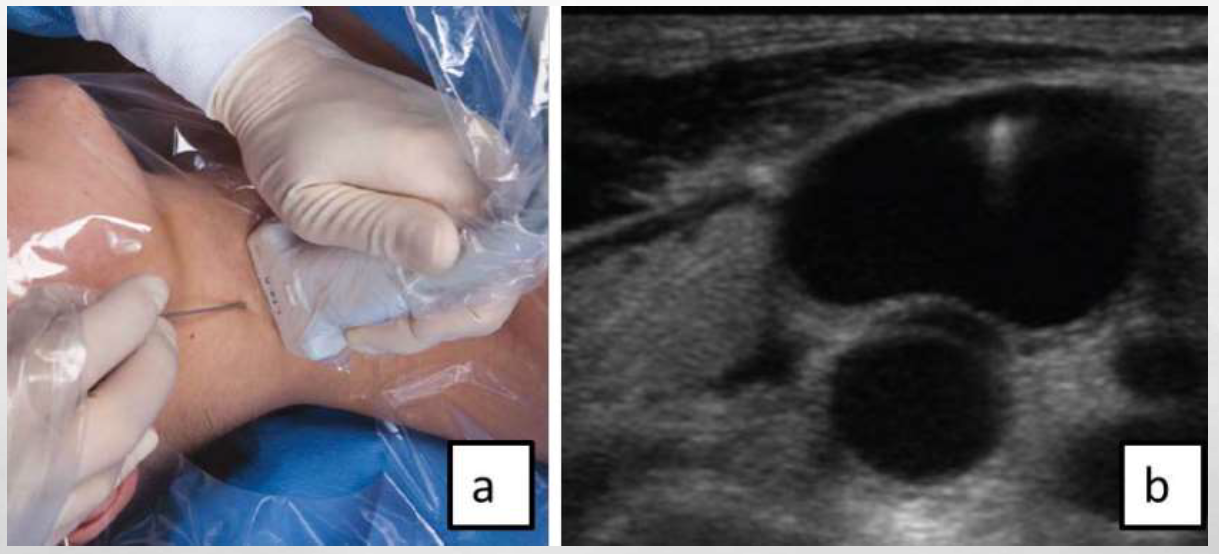
\includegraphics[width=0.7\linewidth]{imagenes/puncion_ecoguiada}
		\caption[Puncion Guiada]{}
		\label{fig:puncionecoguiada}
	\end{figure}
		
	\item Pasaje de \textbf{guía metálica} a través de la aguja; control con RX en región mediastinal.
	
	\begin{figure}[h]
		\centering
		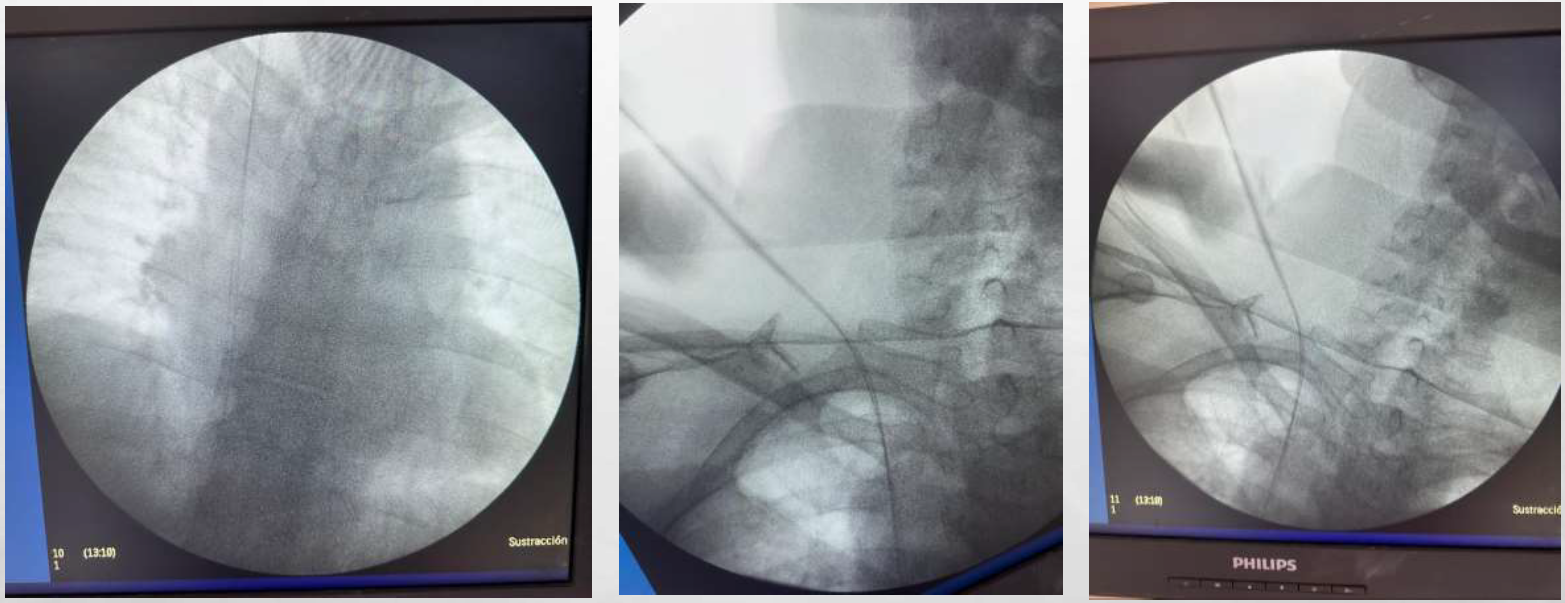
\includegraphics[width=0.7\linewidth]{imagenes/guias_dilatador}
		\caption[Guías y dilatadores]{}
		\label{fig:guiasdilatador}
	\end{figure}
		
	\item Dilatación del acceso venoso con control RX en zona de punción.
	\item Colocación del CDL sobre la guía hasta posición correcta; retirada de la guía con control RX.

	\begin{figure}[h]
		\centering
		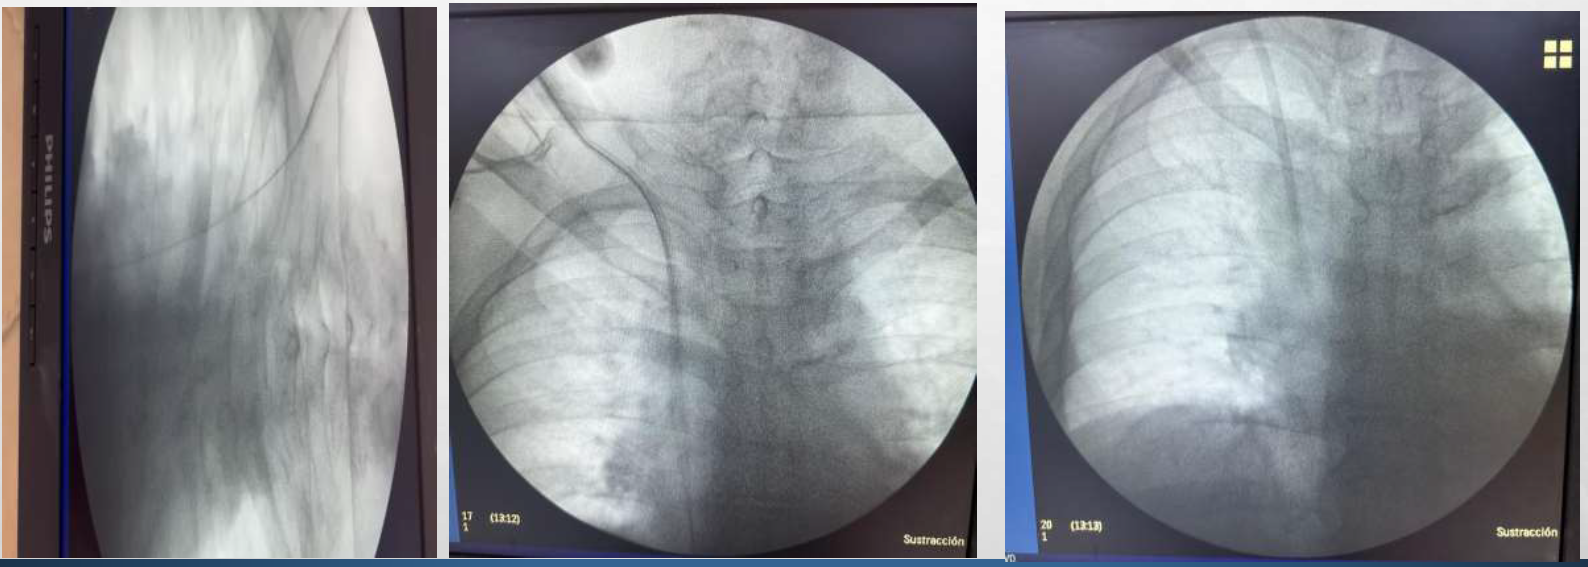
\includegraphics[width=0.7\linewidth]{imagenes/retiro _guia}
		\caption[Retiro de guía]{}
		\label{fig:retiro-guia}
	\end{figure}
	
	
	\item Control final de la \textbf{punta del catéter} en mediastino (nivel de carina / unión VCS--AD).
	\item Prueba de funcionamiento de ambas ramas del catéter.
\end{enumerate}

\subsection*{Catéter Tunelizado (Hickman)}

La fase inicial es idéntica al CDL. Una vez confirmada la posición de la guía, el cirujano realiza adicionalmente:

\begin{enumerate}[noitemsep]
	\item Creación del \textbf{túnel subcutáneo} desde el sitio de punción venosa hasta la salida cutánea planificada.
	\item Pasaje del catéter de silicona por el túnel.
	\item Control radiológico secuencial: guía $\to$ curva $\to$ punta (a nivel de VCS / unión AD).
	
	
	\begin{figure}[h]
		\centering
		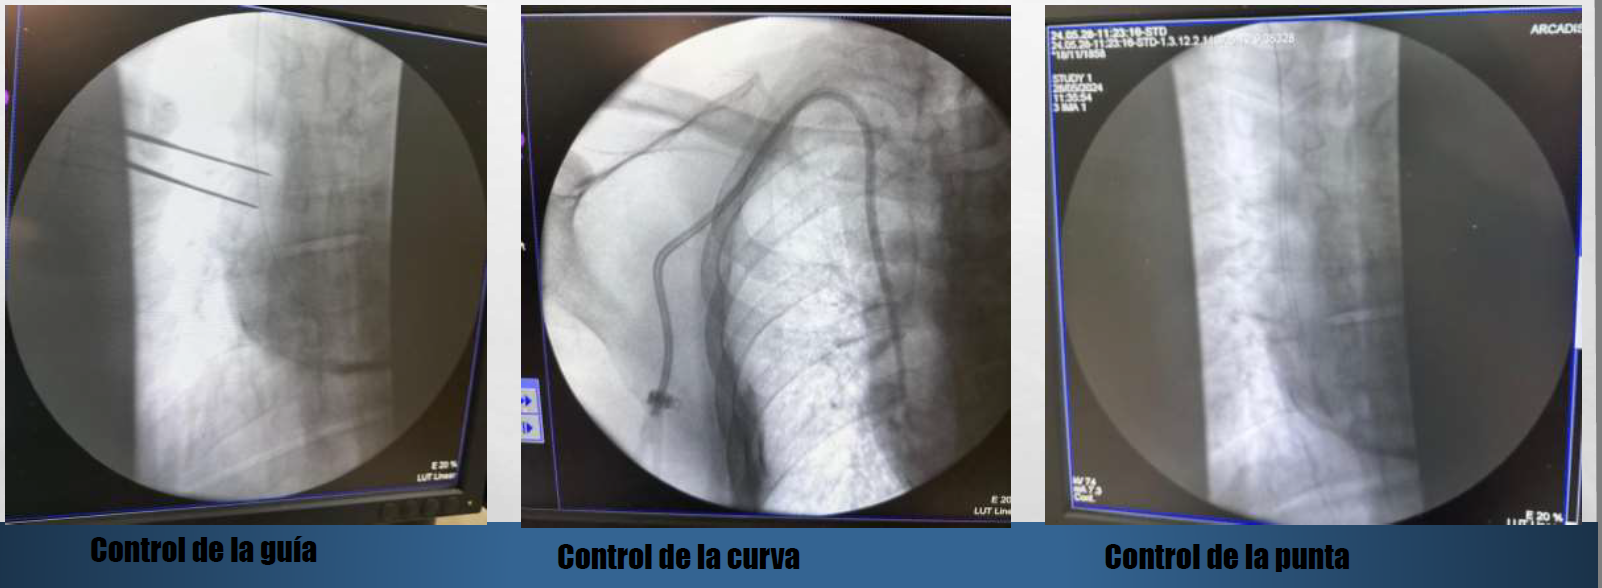
\includegraphics[width=0.7\linewidth]{imagenes/tunelizado_hickman}
		\caption[Controles]{}
		\label{fig:tunelizadohickman}
	\end{figure}
	
	\begin{figure}[h]
		\centering
		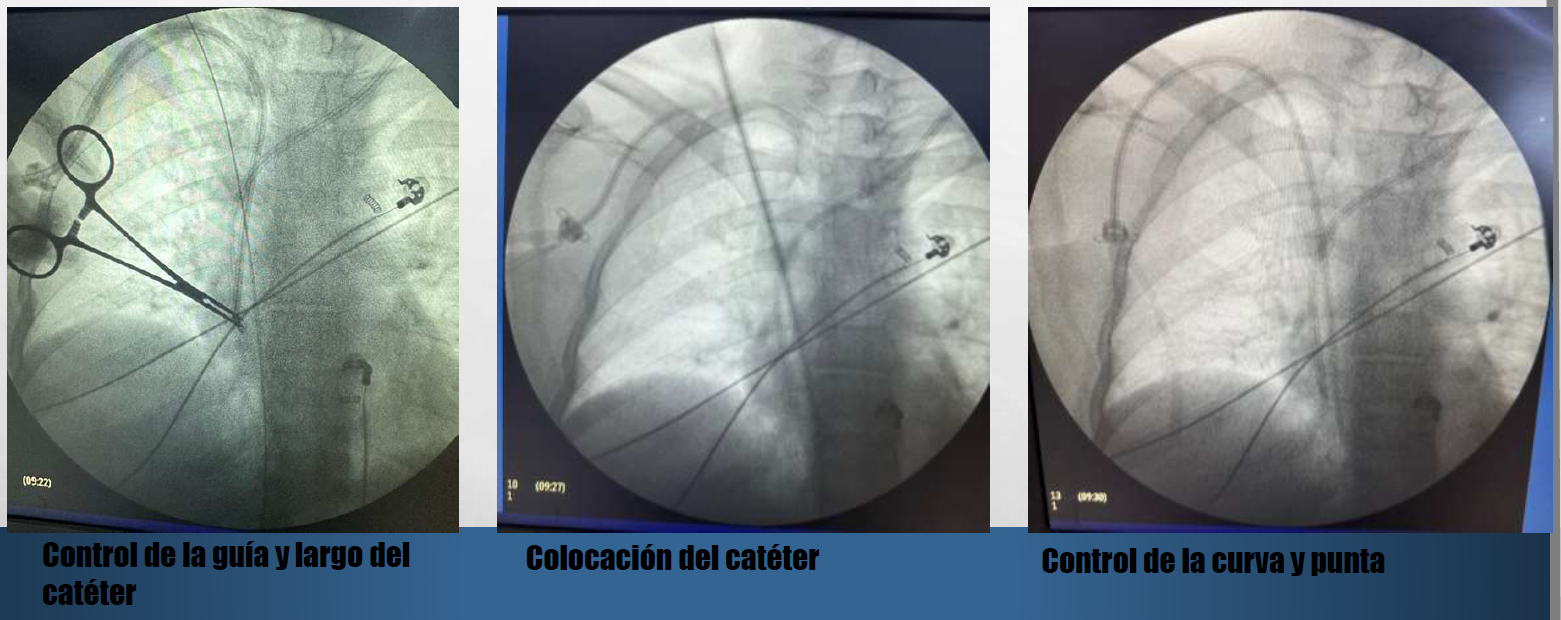
\includegraphics[width=0.7\linewidth]{imagenes/tunelizado_hickman2}
		\caption{}
		\label{fig:tunelizadohickman2}
	\end{figure}
	
\end{enumerate}

\subsubsection{Ubicación de la punta del catéter:}

\begin{itemize}
	\item Se controla por Rx en la vena Cava superior a nivel de la Carina o de unión entre la vena Cava superior y Aurícula derecha.
	
	\item La localización 1/3 superior de vena Cava superior y tronco Braquiocefálico, se asocia a riesgos de trombosis.
	
	\item Dentro de la aurícula puede ocasionar arritmia, trombosis o perforación cardíaca si esta por tiempo prolongado
\end{itemize}

\subsection*{Catéter Gemelar}

Se realizan \textbf{dos punciones independientes} en el mismo vaso. Se colocan dos guías simultáneamente, se controla la posición de ambas, se dilatan los accesos y se insertan los catéteres con las \textbf{puntas a diferente altura} para evitar recirculación.

\begin{figure}[h]
	\centering
	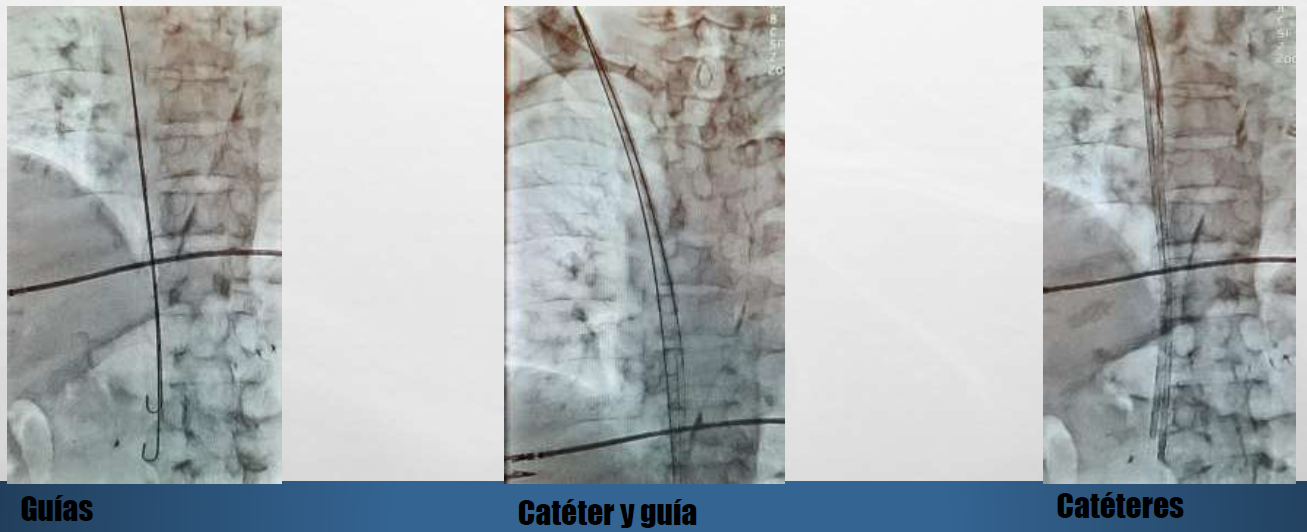
\includegraphics[width=1\linewidth]{imagenes/gemelar1}
	\caption{}
	\label{fig:gemelar1}
\end{figure}

\begin{figure}[h]
	\centering
	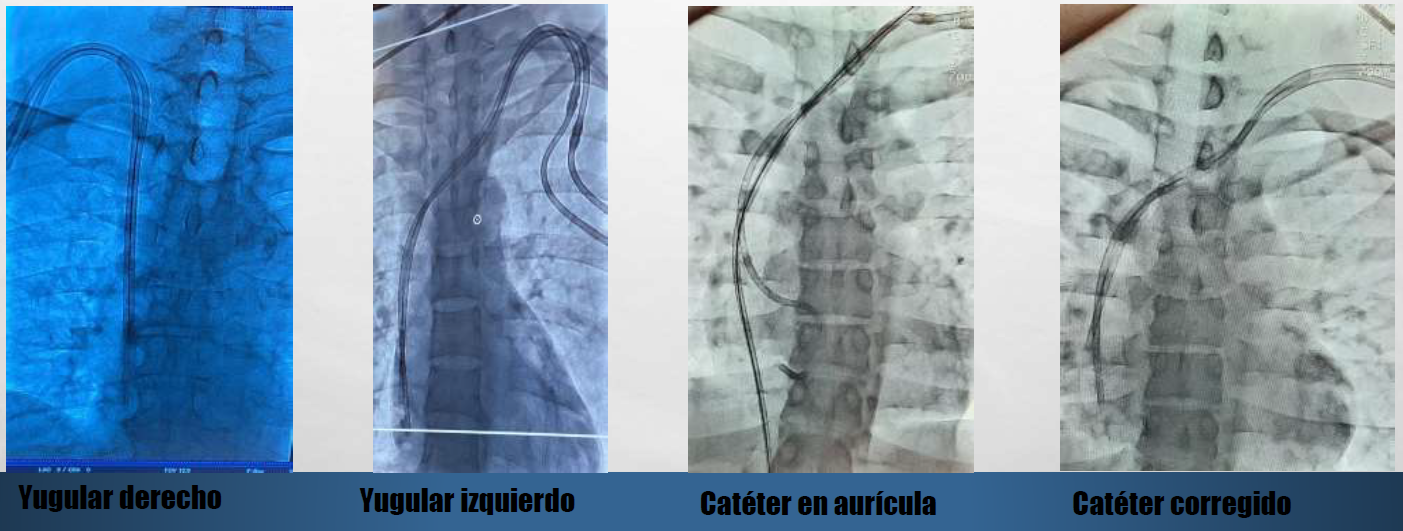
\includegraphics[width=1\linewidth]{imagenes/gemelar2}
	\caption{}
	\label{fig:gemelar2}
\end{figure}



\subsection*{Port-a-Cath}

\begin{enumerate}[noitemsep]
	\item Fase inicial idéntica al CDL (punción, guía, dilatación).
	\item El cirujano realiza un \textbf{bolsillo subcutáneo} en la región del pectoral mayor para alojar el reservorio.
	\item El catéter se tuneliza por vía subcutánea desde el bolsillo hasta el sitio de punción venosa y se conecta al reservorio.
	\item Control radiológico de punta y curvatura para confirmar que el catéter \textbf{no colapse}.
\end{enumerate}


\begin{figure}[h]
	\centering
	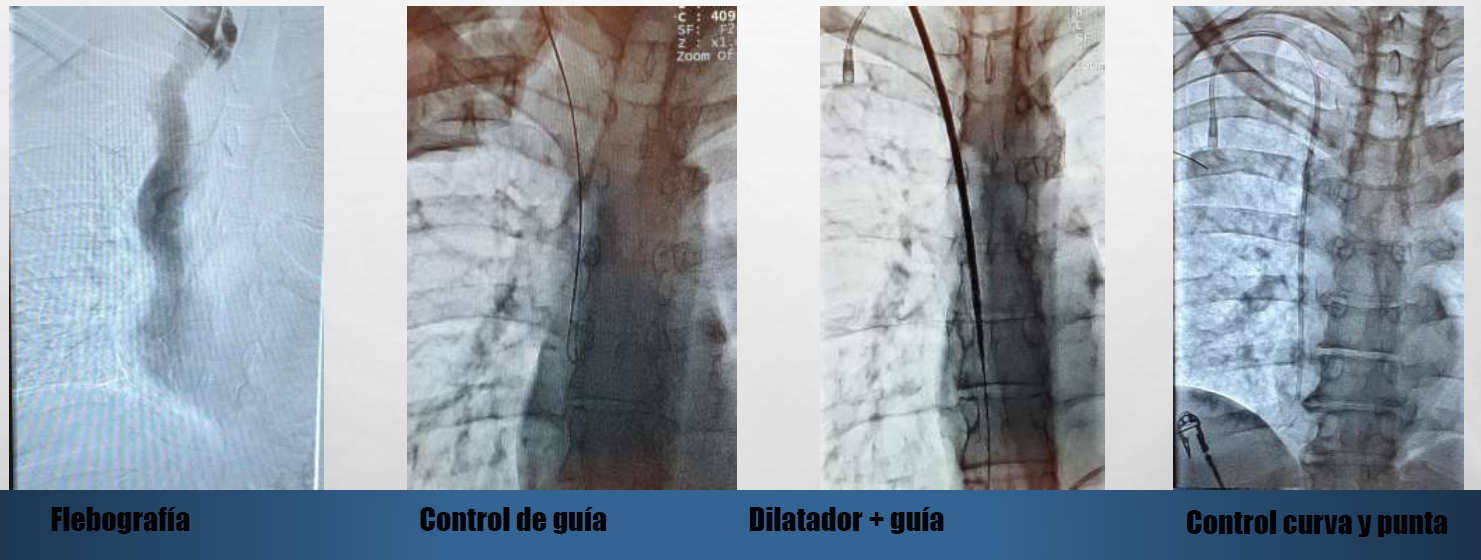
\includegraphics[width=1\linewidth]{imagenes/portacath}
	\caption{}
	\label{fig:portacath}
\end{figure}


\subsubsection{Complicaciones:}
\begin{itemize}
	\item kinking (angulo cerrado de la curva).
	\item Catéter pellizcado.
	\item Neumotorax.
	\item Hemotorax.
\end{itemize}

\clearpage


% ============================================================
%  SECCIÓN 6 --- FISTULOGRAFÍA
% ============================================================
\section*{Fistulografía (FAV)}

Cuando una FAV deja de funcionar (obstrucción), el licenciado en imagenología interviene realizando una \textbf{fistulografía diagnóstica}:

\begin{itemize}[noitemsep]
	\item Adquisición en \textbf{DSA} a 3--6 imágenes/segundo; se aumenta la cadencia para evaluar la dinámica de flujo.
	\item La mayoría de las FAV son \textbf{humerocefálicas o humerobasílicas}; se realizan \textbf{dos enfoques de frente}:
	\begin{enumerate}[noitemsep]
		\item Desde el \textbf{pliegue del codo} (mostrando la aguja de punción) hasta la \textbf{axila inclusive}.
		\item Desde la \textbf{axila} hasta la desembocadura de la VCS en la aurícula derecha.
	\end{enumerate}
	\item Realizado el diagnóstico, el \textbf{cirujano vascular} evaluará el tratamiento (angioplastia, revisión quirúrgica, etc.).
\end{itemize}


\begin{figure}[h]
	\centering
	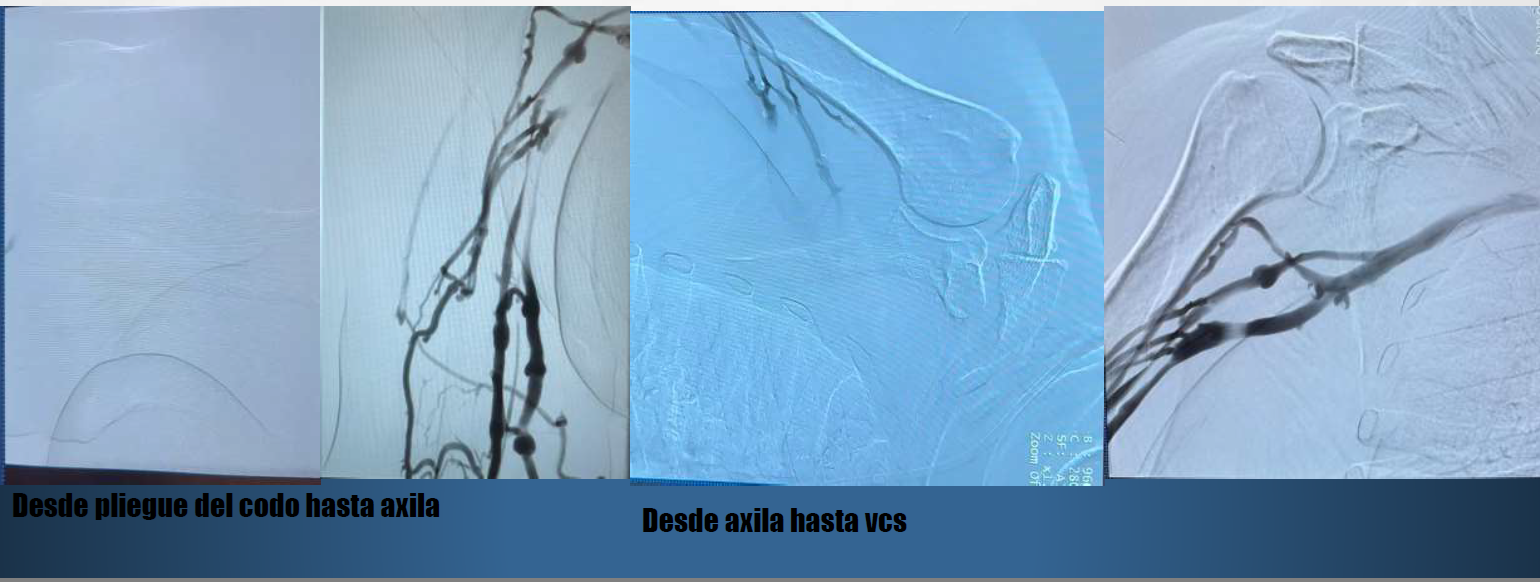
\includegraphics[width=1\linewidth]{imagenes/fistulo}
	\caption{}
	\label{fig:fistulo}
\end{figure}



\subsection*{Filtro de Vena Cava Inferior (FVCI)}

Dispositivo mecánico implantado para \textbf{prevenir embolismos pulmonares} cuando no es posible una anticoagulación adecuada. Los trombos, generados en venas de MMSS o MMII, pueden migrar hacia los pulmones provocando disnea, dolor torácico o muerte.

\begin{enumerate}[noitemsep]
	\item Acceso por vía \textbf{yugular o femoral}; avance de guía hasta VCI abdominal.
	\item Inyección de \textbf{medio de contraste yodado} para identificar la altura de las \textbf{venas renales} (marca en sustracción DSA).
	\item Avance del sistema liberador hasta posición \textbf{infrarenal}.
	\item Liberación del filtro: se expande y ancla a la pared del vaso.
	\item Control final de ubicación con RX.
\end{enumerate}


\clearpage
% ============================================================
%  CIERRE --- ESQUEMA MENTAL FINAL
% ============================================================
\section*{Esquema Mental --- Repaso Final}

\begin{cajakeypoints}
	\begin{center}
		\textbf{\color{azulprincipal}
			Indicación clínica $\rightarrow$ Elección del tipo de CVC $\rightarrow$ Punción eco guiada $\rightarrow$ Seldinger $\rightarrow$ Control RX de punta}\\[0.4em]
		\textbf{\color{naranjadestacado}
			La punta siempre debe quedar en VCS a nivel de carina --- nunca dentro de la aurícula.}\\[0.3em]
		CDL = transitorio, mayor infección \quad Tunelizado = largo plazo, menor infección \quad Port-a-Cath = quimioterapia intermitente\\[0.3em]
		Arco en C: ingresa contralateral al lado de punción \quad Fistulografía DSA: 3--6 img/s, 2 enfoques\\[0.3em]
		\textbf{Filtro VCI:} acceso yugular/femoral $\to$ contraste para identificar renales $\to$ colocar infrarenal $\to$ liberar filtro $\to$ control RX
	\end{center}
\end{cajakeypoints}

\vspace{1em}
\hrule
\vspace{0.5em}
{\footnotesize \textit{Fuente: material de clase --- Lic. Germán Boz ---
		Imagenología Especializada I, UdelaR 2025.}}


\end{document}